\documentclass[12pt]{article}   %Prima era \documentclass{softwaredocumetation}

\usepackage{float} % Metti questa riga nel preambolo per utilizzare H immagine e tabelle

% Impostazioni di codifica e lingua
\usepackage[utf8]{inputenc}
\usepackage[italian]{babel}

% Pacchetti per la grafica
\usepackage{graphicx}

% Pacchetto per l'immagine di sfondo (che verrà applicata a tutte le pagine)
\usepackage{background}
\backgroundsetup{
  scale=1,
  angle=0,
  opacity=1,
  contents={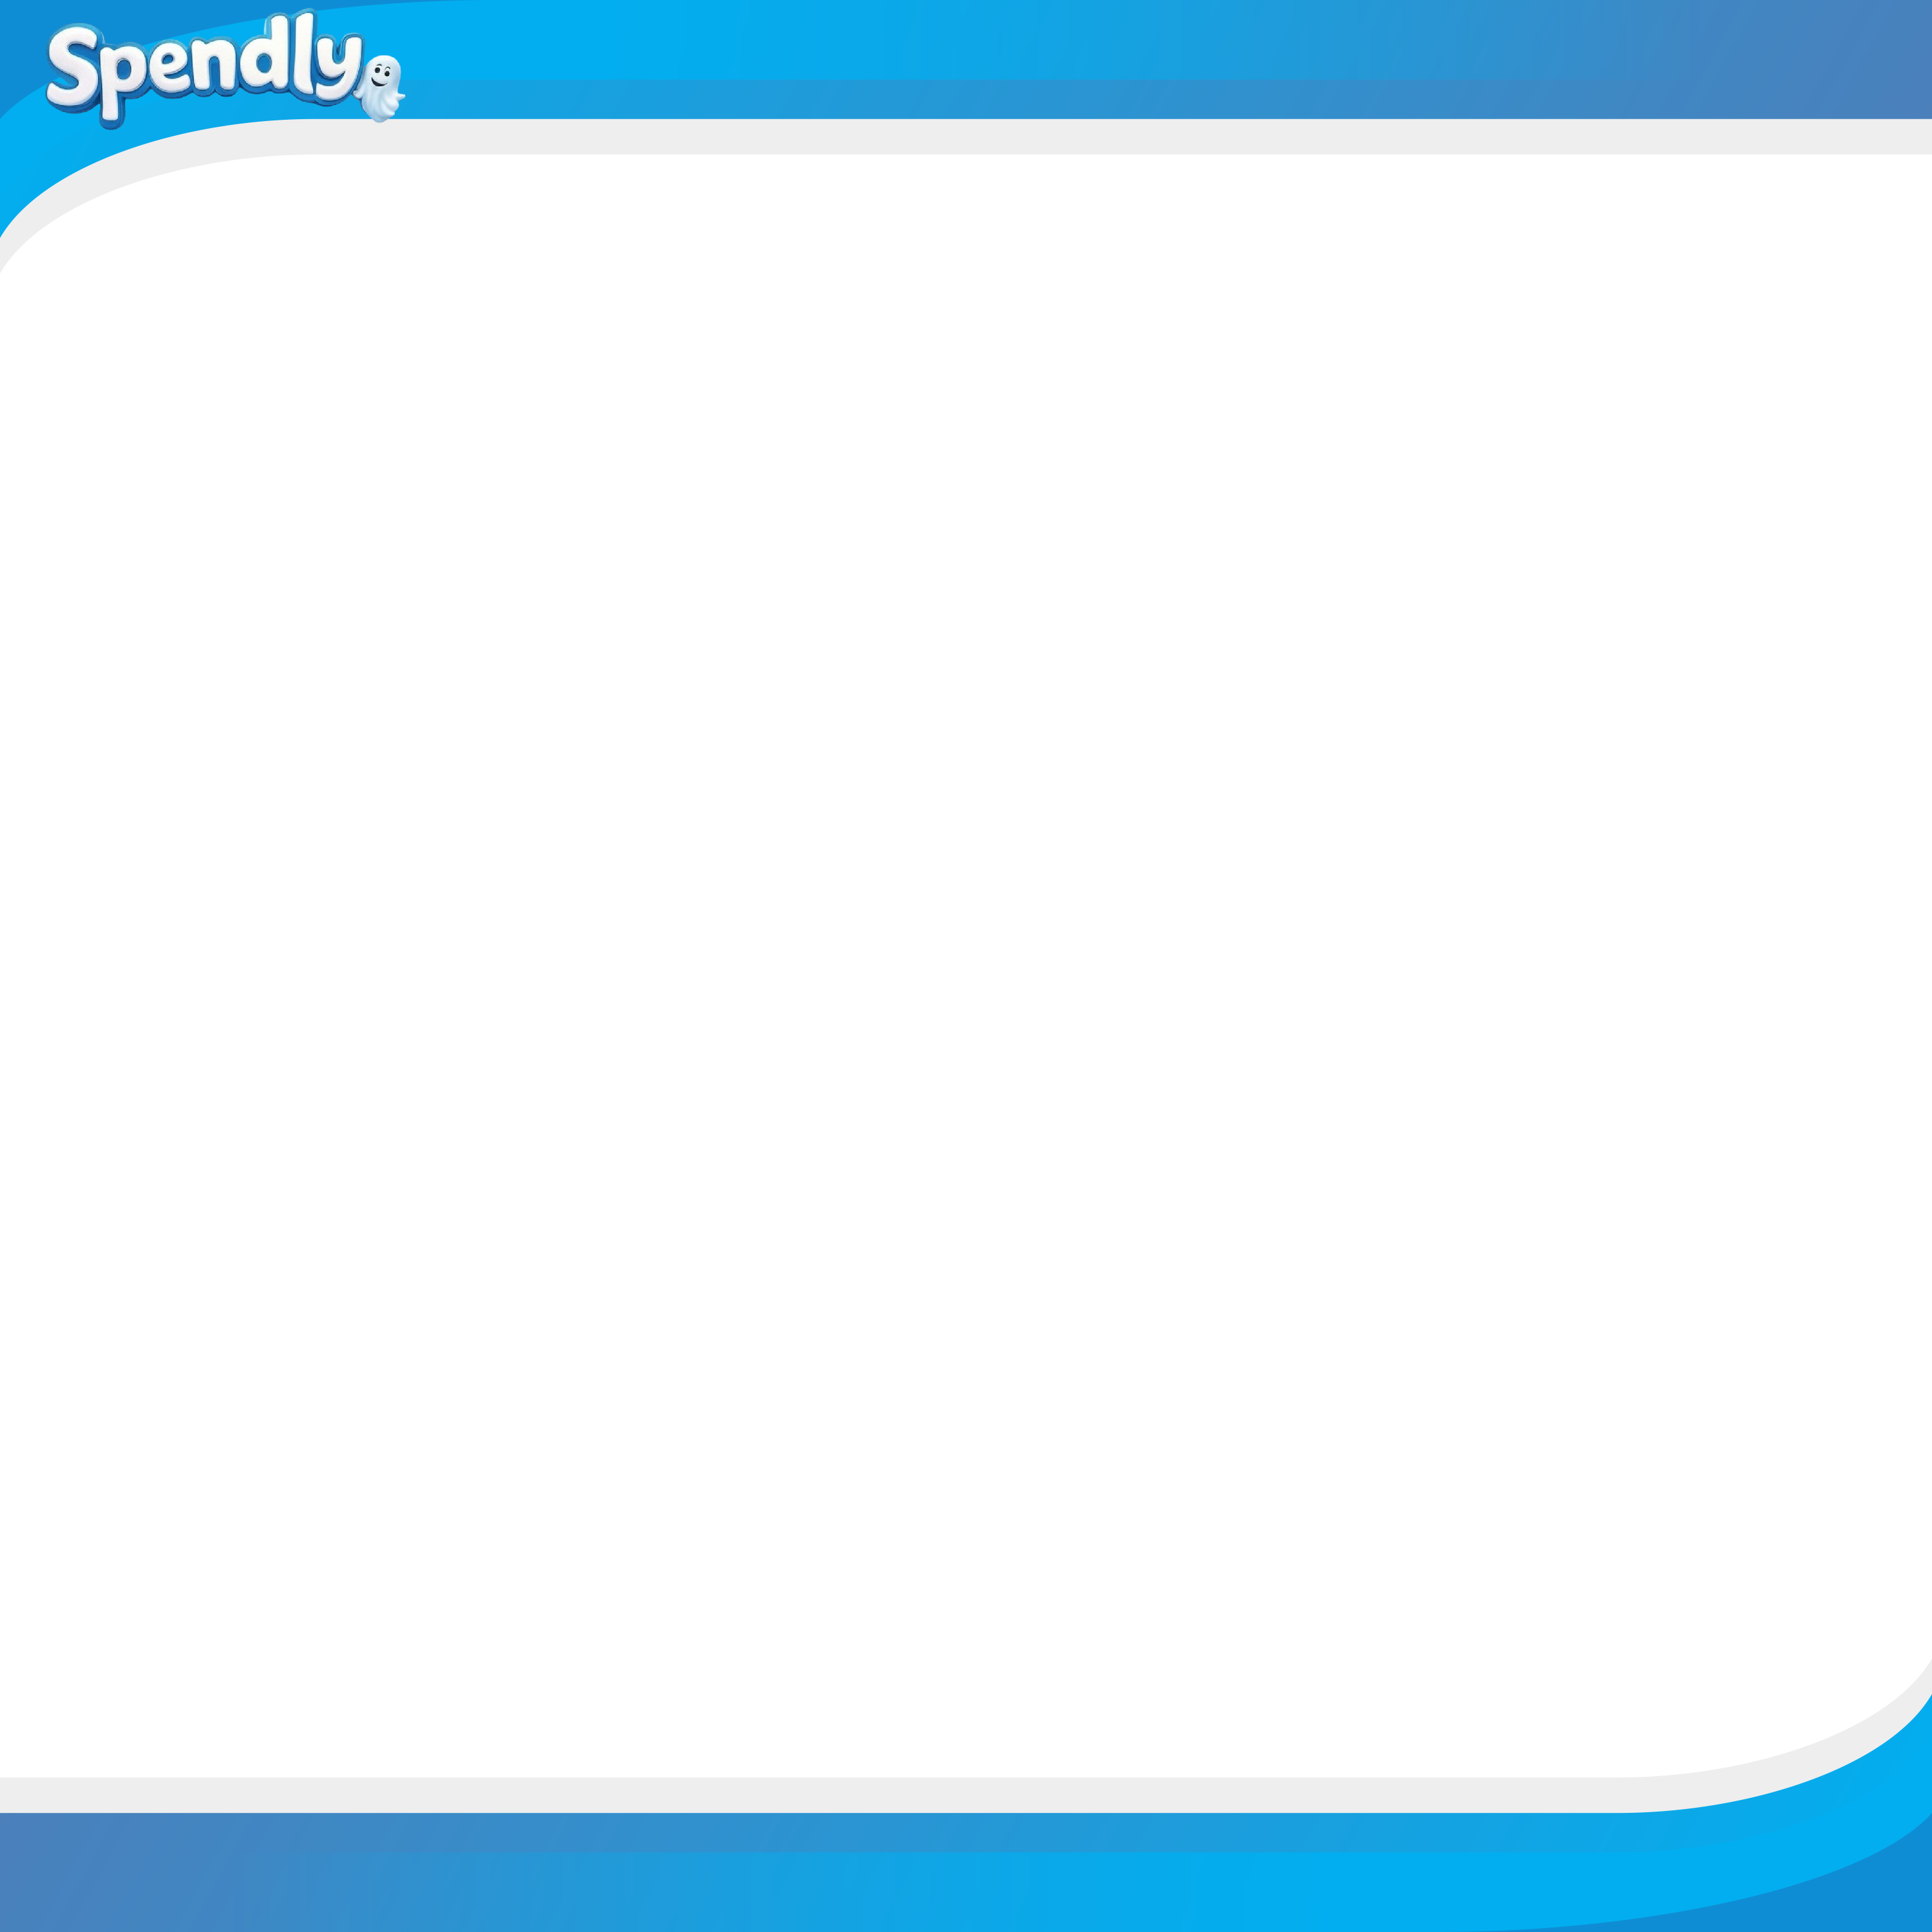
\includegraphics[width=\paperwidth,height=\paperheight]{images/sfondolatex.png}}
}

% Informazioni sul documento
\title{Spendly: Documentazione Tecnica}
\author{Amin Borqal, Loris Iacoban, Diego Rossi}
\date{\today}

\begin{document}

% =======================================================
% TITOLI E MARCHIO NELLA PRIMA PAGINA (Title Page Personalizzata)
% =======================================================
\begin{titlepage}
  \centering
  \vspace*{2cm} % Spazio verticale iniziale

  % Inserimento del logo "Marchio.jpg" centrato
  
\includegraphics[width=0.5\textwidth]{images/Marchio.jpg}\par
  \vspace{1cm}
  
  % Titolo del documento
  {\Huge \bfseries Spendly: Documentazione Tecnica\par}
  \vspace{1cm}
  
  % Autori
  {\Large Amin Borqal, Loris Iacoban, Diego Rossi\par}
  \vspace{1cm}
  
  % Data
  {\Large \today\par}
  \vfill
\end{titlepage}

% =======================================================
% INDICI
% =======================================================
\tableofcontents
\addtocontents{toc}{\protect\thispagestyle{plain}} % Forza lo stile "plain" per l'indice
\newpage
\listoffigures
\listoftables
\newpage 

% =======================================================
% ITERAZIONE 0
% =======================================================
\section{Iterazione 0}


\subsection{Introduzione}

Spendly è una web app progettata per semplificare la gestione delle spese personali e di gruppo, offrendo funzionalità che permettono a singoli utenti, famiglie o gruppi di organizzarsi in modo efficiente.

Con Spendly, è possibile:
\begin{itemize}
    \item Creare gruppi di utenti, dove ciascun membro può registrare le spese effettuate per conto degli altri. L'applicazione calcolerà automaticamente il numero minimo di transazioni necessarie per saldare i debiti all'interno del gruppo.
    \item Impostare avvisi personalizzati per monitorare il livello di spesa del gruppo, fornendo notifiche utili per evitare superamenti del budget condiviso.
\end{itemize}

A livello individuale, ogni utente può:
\begin{itemize}
    \item Visualizzare, registrare e gestire le proprie spese in modo autonomo.
    \item Creare e monitorare un budget di risparmio per pianificare meglio le proprie finanze personali.
\end{itemize}
Grazie a queste funzionalità, Spendly rende la gestione economica più semplice, trasparente ed efficace, sia per singoli utenti che per gruppi.
\newline
\newline
\textbf{Perché scegliere Spendly?}
\\
\\
Spendly è strutturata attorno a una serie di funzionalità che coprono ogni aspetto della gestione delle spese. Queste funzionalità sono state sviluppate con l'obiettivo di offrire la massima flessibilità, sia per gli utenti individuali che per i gruppi di condivisione spese.
Spendly è più di una semplice applicazione di gestione delle spese. È una soluzione completa che integra funzionalità avanzate, come il calcolo automatico dei debiti e la gestione centralizzata delle spese. Questo la rende ideale per ogni tipo di utente, dai gruppi di amici che vogliono semplificare la divisione delle spese, alle famiglie che desiderano tenere sotto controllo i propri budget.
Con una piattaforma sicura, flessibile e facile da usare, Spendly trasforma il modo in cui le persone gestiscono i loro soldi, riducendo lo stress finanziario e migliorando la trasparenza nelle relazioni economiche.
Spendly è lo strumento perfetto per chi desidera una gestione semplice, efficace e organizzata delle spese. Con funzionalità pensate per rispondere alle esigenze di utenti individuali e gruppi, questa web-app rappresenta una soluzione innovativa e accessibile per migliorare la vita quotidiana di chiunque voglia un controllo totale sulle proprie finanze.
\newpage
\subsection{Requisiti}
Il sistema deve soddisfare i seguenti requisiti funzionali e non funzionali:
\begin{itemize}
    \item \textbf{Requisiti Funzionali}:
    \begin{itemize}
        \item Gli utenti devono poter registrarsi e autenticarsi al sistema.
        \item Gli utenti devono poter aggiungere, modificare e cancellare le proprie spese.
        \item Gli utenti devono poter creare gruppi e gestire le spese condivise.
        \item Il sistema deve calcolare automaticamente il bilancio dei debiti tra i membri del gruppo.
    \end{itemize}
    \item \textbf{Requisiti Non Funzionali}:
    \begin{itemize}
        \item L'applicazione deve essere intuitiva e facile da usare.
        \item Il sistema deve garantire la sicurezza dei dati personali degli utenti.
        \item Le transazioni devono essere sincronizzate in tempo reale tra tutti i dispositivi degli utenti.
    \end{itemize}
\end{itemize}

\newpage
\subsection{Casi d'Uso}

    \begin{figure}[h]
        \centering
        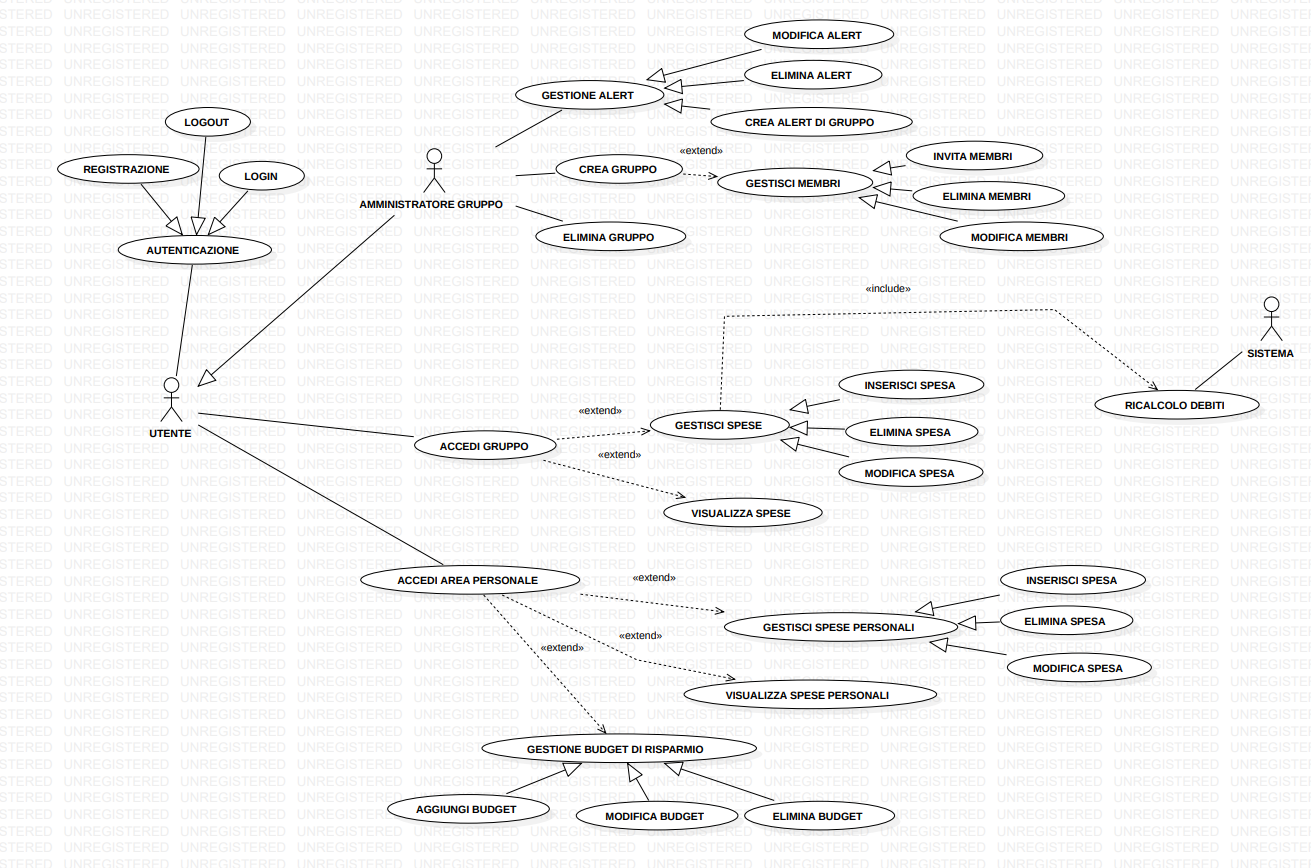
\includegraphics[scale=0.6]{images/casousoprova.png}
        \caption{Diagramma casi d'uso }
    \end{figure}

Di seguito sono riportati i casi d'uso in figura:
\begin{itemize}
    \item \textbf{UC1 - Login}: Come utente, voglio poter accedere al mio account per gestire le mie spese.
    \item \textbf{UC2 - Registrazione}: Come nuovo utente, voglio potermi registrare al sistema per iniziare a usare la web-app.
    \item \textbf{UC3 - Logout}: Voglio poter terminare la mia sessione.
    \item \textbf{UC4 - Crea alert di gruppo}: Come utente amministratore di un gruppo spesa voglio poter inserire un alert, dove un alert è un avviso che ci permette di avvisare se si sta raggiungendo una soglia limite di spesa.
    \item \textbf{UC5 - Modifica alert}: Voglio poter modificare i valori dell'alert.
    \item \textbf{UC6 - Elimina alert}: Voglio poter eliminare l'alert. 
    \item \textbf{UC7 - Crea gruppo}: Voglio poter creare un gruppo di condivisione spese. 
    \item \textbf{UC8 - Invita memebri}: Voglio come amministratore invitare membri nel gruppo di spese.
    \item \textbf{UC9 - Elimina membri}: Voglio come amministratore poter eliminare membri del gruppo di spese.
    \item \textbf{UC10 - Modifica membri}: Voglio come amministratore modificare i membri nel gruppo di spese.
    \item \textbf{UC11 - Elimina gruppo}: Voglio poter eliminare un gruppo di condivisione spese. 
    \item \textbf{UC12 - Accedi gruppo}: Voglio poter accedere ad un gruppo di condivisione spese. 
    \item \textbf{UC13 - Inserisci spesa}: Voglio poter inserire una spesa di gruppo.
    \item \textbf{UC14 - Elimina spesa}: Voglio poter eliminare una spesa di gruppo.
    \item \textbf{UC15 - Modifica spesa}: Voglio poter modificare una spesa di gruppo.
    \item \textbf{UC16 - Visualizza spese}: Voglio poter visualizzare le spesa di gruppo.
    \item \textbf{UC17 - Ricalcolo debiti}: Voglio poter calcolare i debiti.
    \item \textbf{UC18 - Inserisci spesa personale}: Voglio poter inserire una spesa personali.
    \item \textbf{UC19 - Elimina spesa personale}: Voglio poter eliminare una spesa personali.
    \item \textbf{UC20 - Modifica spesa personale}: Voglio poter modificare una spesa personali.
    \item \textbf{UC21 - Visualizza spesa personale}: Voglio poter visualizzare le spesa personali.
    \item \textbf{UC22 - Inserisci budget}: Voglio poter inserire un budget di risparmio.
    \item \textbf{UC23 - Elimina budget}: Voglio poter eliminare un budget di risparmio.
    \item \textbf{UC24 - Modifica budget}: Voglio poter modificare un budget di risparmio.
    \item \textbf{UC25 - Visualizza budget}: Voglio poter visualizzare i budget di risparmio.
\end{itemize}

\section{Architettura}
L'architettura del sistema è basata su un'architettura a microservizi con i seguenti componenti principali:
\begin{itemize}
    \item \textbf{Client/Frontend}: Implementato in React.js, il frontend fornisce un'interfaccia utente intuitiva per la gestione delle spese.
    \item \textbf{API Gateway}: Un punto di ingresso unico per tutte le richieste del client, responsabile dell'instradamento verso i microservizi corretti.
    \item \textbf{Backend (Microservizi)}: I microservizi sono sviluppati in Spring Boot e includono:
    \begin{itemize}
        \item \textbf{Servizio Utente}: Gestisce la registrazione, l'autenticazione e il profilo utente.
        \item \textbf{Servizio Gestione Spese}: Gestisce le operazioni CRUD sulle spese.
        \item \textbf{Servizio Gruppi}: Gestisce la creazione e la modifica dei gruppi.
    \end{itemize}
    \item \textbf{Database}: Utilizzo di PostgreSQL per la gestione dei dati relazionali.
\end{itemize}

\input{Iterazione0/priorità.tex}
%\newpage
\subsection{Topologia del Sistema}

La topologia del sistema è rappresentata nel seguente schema:

\begin{figure}[h]
\centering
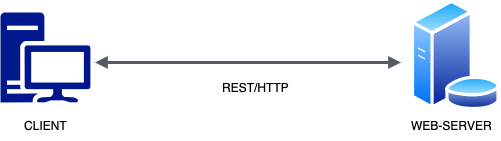
\includegraphics[scale=0.75]{images/topologia.png}
\caption{Diagramma dell’architettura della webapp Spendly}
\end{figure}

Il sistema è basato unicamente su un’architettura \textbf{web}, in cui i client interagiscono con un \textbf{web server} sviluppato in \textbf{Spring Boot}. I client utilizzano un browser, comunicando con il server attraverso \textbf{REST-API HTTP}, con dati in formato \textbf{JSON}. 

\subsubsection{Protocollo HTTP e REST-API}

HTTP è un protocollo di trasferimento ipertestuale che offre un meccanismo semplice e universale per inviare e ricevere dati. È ideale per le nostre REST-API poiché assicura la compatibilità con i browser e l’interscambio di dati in JSON su qualsiasi piattaforma.

\subsubsection{Caratteristiche dell’architettura}

\begin{itemize}
\item \textbf{Scalabilità}: possibilità di scalare l’intero sistema o le singole funzionalità in base alle necessità.
\item \textbf{Modularità}: sviluppo e manutenzione semplificati grazie all’organizzazione delle funzionalità in moduli indipendenti.
\item \textbf{Affidabilità}: eventuali malfunzionamenti in una funzionalità non compromettono l’intero sistema.
\item \textbf{Manutenibilità}: possibilità di aggiornare o sostituire singoli moduli senza interrompere l’operatività complessiva.
\end{itemize}
\newpage
\subsection{Strumenti Utilizzati}

Lo sviluppo del progetto è supportato da una serie di strumenti software che facilitano la progettazione, lo sviluppo, il testing e la gestione del codice. Di seguito, una panoramica dettagliata dei tool impiegati:

\begin{itemize}
    \item \textbf{Visual Studio Code}: IDE (Integrated Development Environment) scelto per lo sviluppo del progetto. VS Code offre un ambiente di sviluppo leggero ma potente, con un ampio supporto per il linguaggio Java e numerose estensioni utili. Tra i plugin utilizzati troviamo:
    \begin{itemize}
        \item \textbf{Spring Boot Extension Pack}: per il supporto avanzato nello sviluppo di applicazioni Spring Boot.
        \item \textbf{Java Extension Pack}: per il supporto completo al linguaggio Java, con funzionalità di autocompletamento, refactoring e debugging.
    \end{itemize}
    
    \item \textbf{Spring Boot}: Framework Java basato su Spring, progettato per lo sviluppo di applicazioni web scalabili e strutturate secondo l’architettura a microservizi. Grazie alla sua configurazione automatica e al supporto integrato per REST API, Spring Boot semplifica la gestione del backend e garantisce un’elevata manutenibilità del codice.
    
    \item \textbf{PostgreSQL}: Sistema di gestione di database relazionale (RDBMS) scelto per la sua affidabilità, scalabilità e aderenza agli standard SQL. PostgreSQL supporta transazioni ACID (Atomicità, Coerenza, Isolamento, Durabilità) ed è ottimizzato per operazioni complesse e interrogazioni avanzate. Il database è stato configurato per garantire prestazioni elevate e sicurezza dei dati.

    \item \textbf{Postman}: Strumento essenziale per il testing delle API REST sviluppate con Spring Boot. Consente di effettuare richieste HTTP, validare le risposte del server e automatizzare test, facilitando così il debug e l’integrazione tra i diversi componenti del sistema.

    \item \textbf{Grok AI}: Tecnologia avanzata per la generazione automatica di immagini basata su intelligenza artificiale. Grok AI viene utilizzato per creare rappresentazioni visive intuitive e schematiche di concetti complessi, supportando la documentazione e la comunicazione grafica del progetto.

    \item \textbf{JUnit 4}: Framework per il testing unitario in Java, impiegato per validare il corretto funzionamento delle classi e dei metodi sviluppati. L’uso di test automatizzati consente di rilevare tempestivamente eventuali errori e di garantire la robustezza del codice.

    \item \textbf{JGraphT}: Libreria Java dedicata alla modellazione e alla gestione di strutture dati basate su grafi. Utilizzata per la rappresentazione e la manipolazione di relazioni complesse all’interno del sistema.

    \item \textbf{CodeMR}: Strumento avanzato per l’analisi della qualità del codice Java e la visualizzazione delle metriche software. CodeMR consente di valutare la complessità del codice, individuare problemi di design e migliorare la manutenibilità del progetto.

    \item \textbf{GitHub}: Piattaforma per il versionamento del codice basata su Git, utilizzata per il controllo delle versioni e la collaborazione tra gli sviluppatori. Grazie a GitHub, è possibile tracciare le modifiche al codice, gestire le revisioni e garantire un workflow ordinato ed efficiente. 

    \item \textbf{GitHub Desktop}: Applicazione con interfaccia grafica che semplifica l’interazione con il repository GitHub direttamente dal PC. Permette di eseguire operazioni di commit, push e pull senza dover utilizzare la riga di comando, facilitando la gestione del codice per gli sviluppatori.

    \item \textbf{StarUML}: Software utilizzato per la modellazione di diagrammi UML (Unified Modeling Language), fondamentale nella fase di progettazione dell'architettura del sistema. StarUML consente di rappresentare visivamente classi, casi d’uso e flussi operativi.

    \item \textbf{diagrams.net}: Applicazione web per la creazione di diagrammi e schemi con notazione libera. Utilizzata per rappresentare graficamente flussi di dati, processi e architetture software, facilitando la comprensione e la condivisione delle informazioni progettuali.

    \item \textbf{WhatsApp}: Applicazione di messaggistica utilizzata come strumento di comunicazione interna tra i membri del team. Attraverso WhatsApp, è possibile coordinare le attività di sviluppo, discutere problemi tecnici e organizzare riunioni in tempo reale, garantendo un flusso comunicativo rapido ed efficiente.

    \item \textbf{Telegram}: Applicazione di messaggistica utilizzata dal team per discussioni tecniche e condivisione rapida di documenti, codice e aggiornamenti di progetto. Grazie ai suoi bot e alle funzionalità avanzate di gestione dei gruppi, Telegram rappresenta uno strumento utile per il coordinamento del lavoro.

\end{itemize}


% =======================================================
% ITERAZIONE 1
% =======================================================
\newpage
\section{Iterazione 1}

\subsection{Casi d'Uso Implementati }

In questa iterazione sono stati sviluppati i seguenti casi d’uso ritenuti prioritari per lo sviluppo di \textbf{Spendly}.

\begin{table}[H]
    \centering
    \begin{tabular}{|c|l|}
    \hline
    \textbf{ID} & \textbf{Titolo} \\ \hline
    UC1 & Login\\ \hline
    UC2 & Registrazione \\ \hline
    UC3 & Logout \\ \hline
    UC7 & Crea gruppo \\ \hline
    UC8 & Invita membri \\ \hline
    UC9 & Elimina membri \\ \hline
    UC10 & Modifica membri \\ \hline
    UC11 & Elimina gruppo \\ \hline
    UC12 & Accedi gruppo \\ \hline
    \end{tabular}
    \caption{Iterazione1}
\end{table}

\subsubsection{UC1: Login}
\textbf{Attori}: Utente, Sistema.
\\
\\
\textbf{Descrizione}: L'utente può autenticarsi nel sistema per accedere al proprio account.
\\
\\
\textbf{Flusso degli eventi}:
\begin{enumerate}
    \item L'utente accede alla pagina di login.
    \item Inserisce email e password.
    \item Il sistema verifica le credenziali e autentica l'utente.
    \item L'utente viene reindirizzato alla dashboard.
\end{enumerate}

\subsubsection{UC2: Registrazione}
\textbf{Attori}: Utente, Sistema.
\\
\\
\textbf{Descrizione}: Un nuovo utente può registrarsi creando un account.
\\
\\
\textbf{Flusso degli eventi}:
\begin{enumerate}
    \item L'utente accede alla pagina di registrazione.
    \item Inserisce nome, email e password.
    \item Il sistema verifica che l’email non sia già registrata.
    \item Se la verifica è superata, il sistema crea l’account e lo memorizza.
    \item L'utente viene reindirizzato alla dashboard.
\end{enumerate}

\subsubsection{UC3: Logout}
\textbf{Attori}: Utente, Sistema.
\\
\\
\textbf{Descrizione}: L'utente può terminare la sessione ed effettuare il logout.
\\
\\
\textbf{Flusso degli eventi}:
\begin{enumerate}
    \item L'utente clicca su "Logout".
    \item Il sistema invalida la sessione e mostra la schermata di login.
\end{enumerate}

\subsubsection{UC7: Creazione Gruppo}
\textbf{Attori}: Utente amministratore, Sistema.
\\
\\
\textbf{Descrizione}: L’utente può creare un nuovo gruppo di spese per la condivisione con altri membri.
\\
\\
\textbf{Flusso degli eventi}:
\begin{enumerate}
    \item L’utente clicca su "Crea Gruppo".
    \item Inserisce il nome del gruppo e una descrizione opzionale.
    \item Il sistema crea il gruppo e assegna l’utente come amministratore.
    \item L'utente viene reindirizzato alla pagina del gruppo.
\end{enumerate}

\subsubsection{UC8: Invita Membri}
\textbf{Attori}: Utente amministratore, Sistema.
\\
\\
\textbf{Descrizione}: L’amministratore di un gruppo può invitare altri utenti a unirsi al gruppo di spese.
\\
\\
\textbf{Flusso degli eventi}:
\begin{enumerate}
    \item L’amministratore accede alla pagina del gruppo.
    \item Clicca su "Invita Membri" e inserisce l’email degli utenti da invitare.
    \item Il sistema invia un’email con l’invito e memorizza la richiesta.
    \item Gli utenti ricevono l’invito e possono accettarlo per entrare nel gruppo.
\end{enumerate}

\subsubsection{UC9: Elimina Membri}
\textbf{Attori}: Utente amministratore, Sistema.
\\
\\
\textbf{Descrizione}: L’amministratore di un gruppo può rimuovere un membro dal gruppo.
\\
\\
\textbf{Flusso degli eventi}:
\begin{enumerate}
    \item L’amministratore accede alla lista dei membri del gruppo.
    \item Seleziona il membro da rimuovere e clicca su "Elimina".
    \item Il sistema rimuove il membro e aggiorna la lista.
\end{enumerate}

\subsubsection{UC10: Modifica Membri}
\textbf{Attori}: Utente amministratore, Sistema.
\\
\\
\textbf{Descrizione}: L’amministratore di un gruppo può modificare i dettagli dei membri (ad esempio assegnare nuovi ruoli).
\\
\\
\textbf{Flusso degli eventi}:
\begin{enumerate}
    \item L’amministratore accede alla lista dei membri.
    \item Seleziona un membro e modifica i dettagli (es. ruolo nel gruppo).
    \item Il sistema aggiorna i dati e notifica il cambiamento.
\end{enumerate}

\subsubsection{UC11: Eliminazione Gruppo}
\textbf{Attori}: Utente amministratore, Sistema.
\\
\\
\textbf{Descrizione}: L’amministratore di un gruppo può eliminare definitivamente un gruppo di spese.
\\
\\
\textbf{Flusso degli eventi}:
\begin{enumerate}
    \item L’amministratore accede alle impostazioni del gruppo.
    \item Clicca su "Elimina Gruppo".
    \item Il sistema chiede conferma prima di procedere.
    \item Se confermato, il gruppo e tutte le sue spese vengono eliminate.
\end{enumerate}

\subsubsection{UC12: Accesso a un Gruppo}
\textbf{Attori}: Utente, Sistema.
\\
\\
\textbf{Descrizione}: Un utente può accedere a un gruppo di spese a cui è stato invitato.
\\
\\
\textbf{Flusso degli eventi}:
\begin{enumerate}
    \item L'utente riceve un invito via email o notifica nell’app.
    \item Clicca sul link di invito e accede alla web-app.
    \item Il sistema verifica la validità dell’invito e aggiunge l’utente al gruppo.
    \item L'utente viene reindirizzato alla pagina del gruppo.
\end{enumerate}
\newpage
\subsection{UML Component Diagram}


\begin{center}
    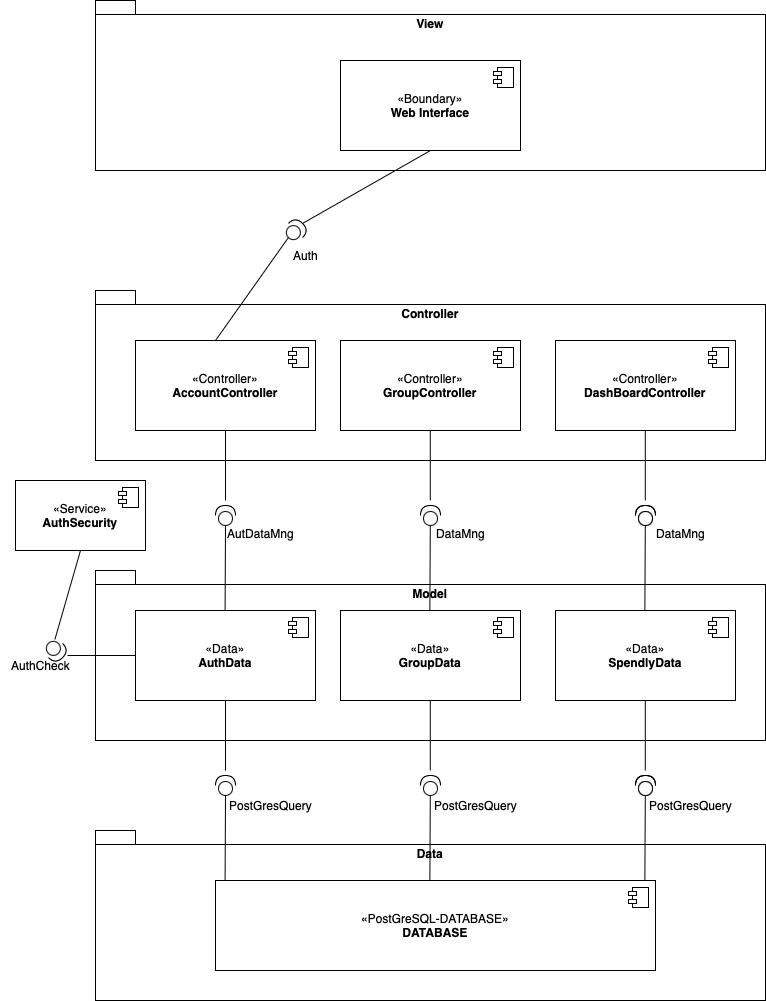
\includegraphics[scale=0.45]{images/ComponentDiagramV1.1.png}

\end{center}

Partendo dai casi d’uso selezionati per questa iterazione e procedendo con l’utilizzo delle euristiche di design, è stato possibile progettare l’architettura software del sistema \textbf{Spendly}.  
I componenti sono organizzati secondo il pattern \textbf{MVC (Model-View-Controller)}, con la suddivisione in:
\begin{itemize}
    \item \textbf{Boundary} - Interfaccia utente, responsabile dell'interazione con l'utente finale.
    \item \textbf{Controller} - Gestione logica di business.
    \item \textbf{Model} - Gestione dei dati e accesso al database.
    \item \textbf{Service} - Servizi di sicurezza e autenticazione.
    \item \textbf{Database} - PostgreSQL.
\end{itemize}

\newpage
\subsection{UML Class Diagram per tipi di dato}

\begin{center}
    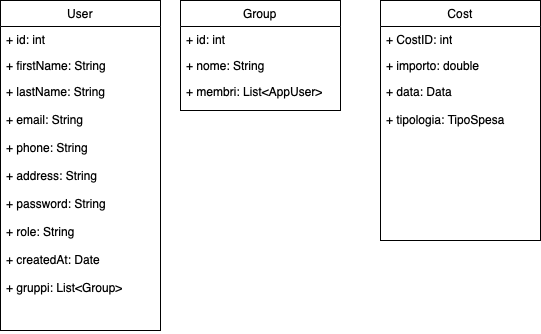
\includegraphics[scale=0.55]{images/TipoDatiClassDiagramV1.1.png}

\end{center}



\newpage
\subsection{Testing}
\subsubsection{Analisi Statica - CodeMR}

L'analisi statica del codice è stata gestita tramite il tool CodeMR.

\begin{figure}[H]
    \centering
    \begin{minipage}{0.45\textwidth}
        \centering
        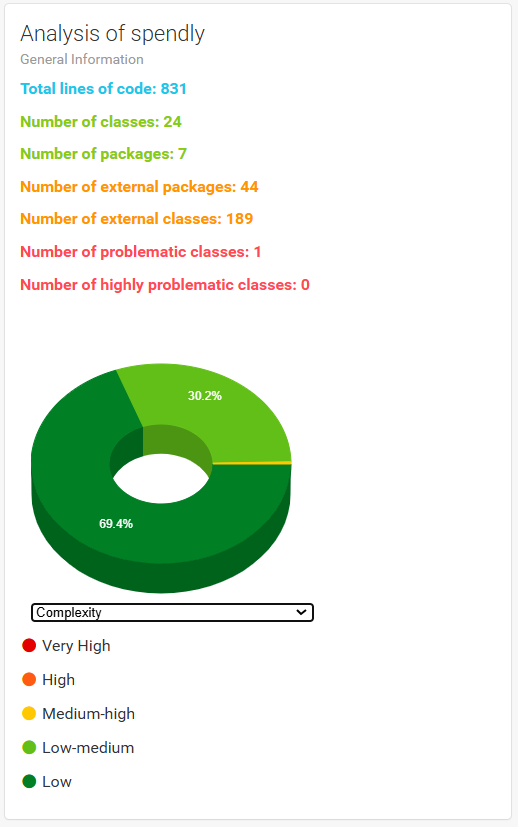
\includegraphics[width=\textwidth]{images/complexity_iter1.png}
        \caption{Complexity}
        \label{fig:Complexity_iterazione1}
    \end{minipage}
    \hfill
    \begin{minipage}{0.45\textwidth}
        \centering
        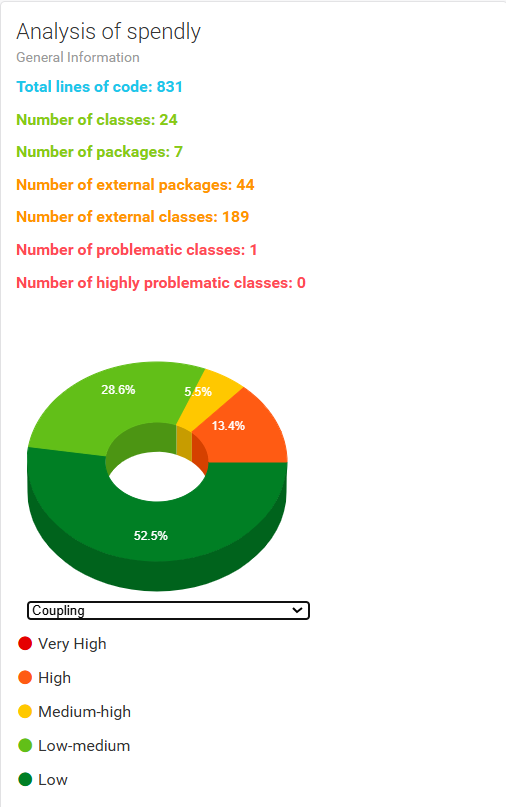
\includegraphics[width=\textwidth]{images/coupling_iter1.png}
        \caption{Coupling}
        \label{fig:Coupling_iterazione1}
    \end{minipage}
\end{figure}

\begin{figure}[H]
    \centering
    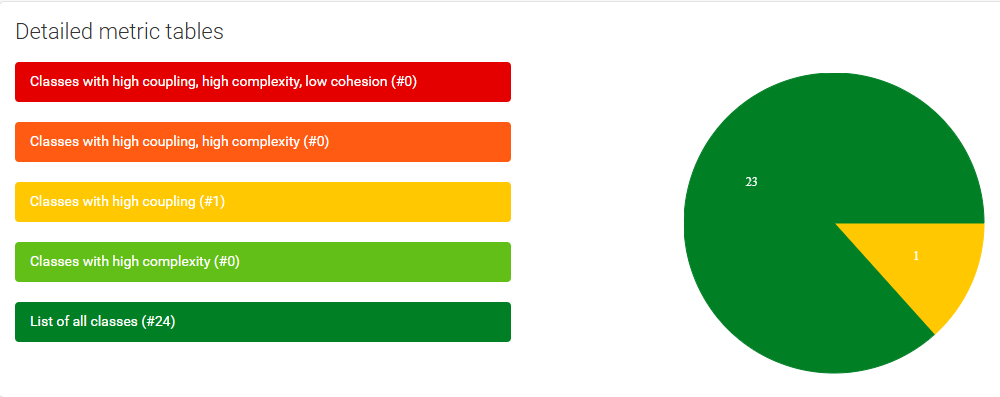
\includegraphics[width=0.9\textwidth]{images/Problem2_iter1.png}
    \caption{Problemi classi}
    \label{fig:Problemi_iterazione1}
\end{figure}

\begin{figure}[H]
    \centering
    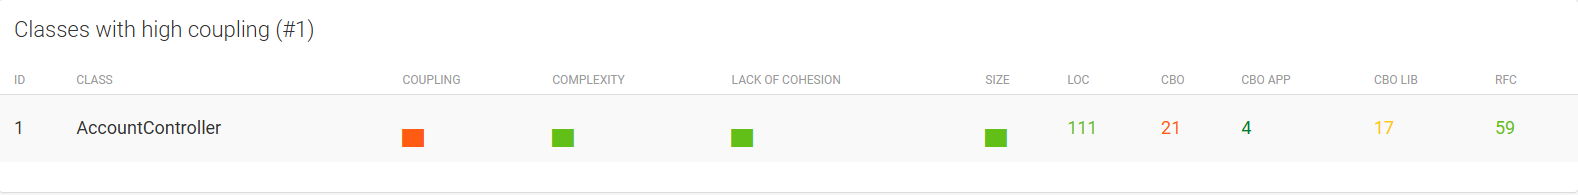
\includegraphics[width=0.9\textwidth]{images/Problem3_iter1.png}
    \caption{Problemi classi 2}
    \label{fig:Problemi_iterazione1}
\end{figure}



\begin{figure}[H]
    \centering
    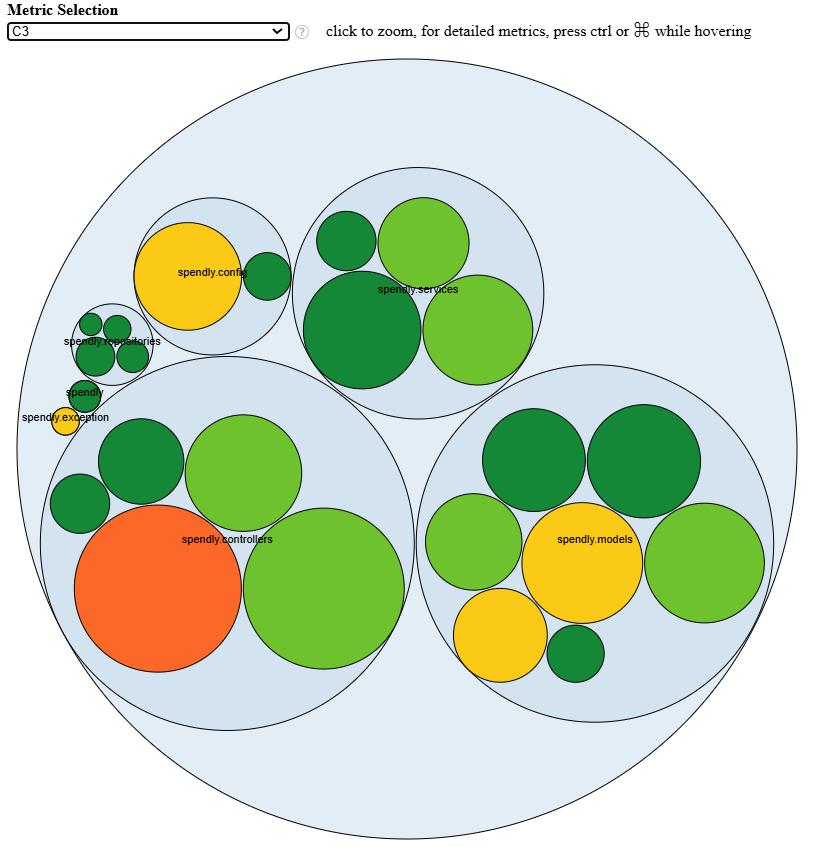
\includegraphics[width=0.9\textwidth]{images/CodeMR_graph2.png}
    \caption{Struttura dei package}
    \label{fig:Package_iterazione1}
\end{figure}


\subsubsection{Analisi Dinamica - JUnit}

L'analisi dinamica del codice è stata condotta utilizzando JUnit per l'esecuzione di test automatizzati sui metodi delle principali classi, e Postman per verificare il corretto funzionamento delle API implementate nei controller.
In particolare, con JUnit sono stati sviluppati test specifici per validare i metodi delle classi relative alla gestione dei gruppi, quali Group, GroupService e GroupController.

\begin{figure}[H]
    \centering
    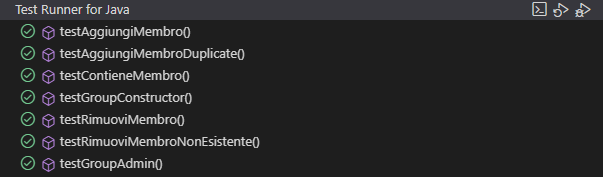
\includegraphics[width=0.9\textwidth]{images/TestGroup.png}
    \caption{Test per la classe Group}
    \label{fig:Group_test}
\end{figure}

\begin{figure}[H]
    \centering
    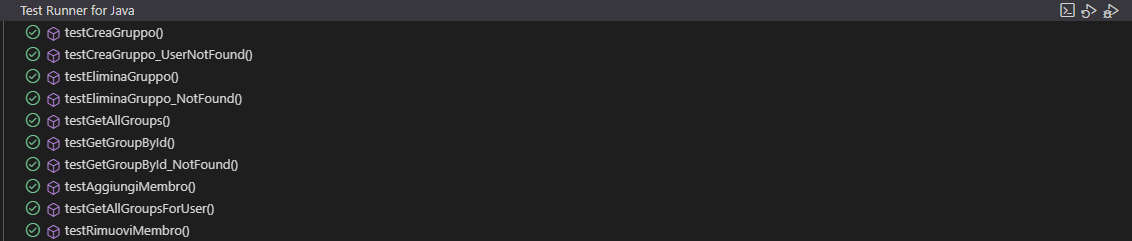
\includegraphics[width=0.9\textwidth]{images/TestGroupService.png}
    \caption{Test per la classe GroupService}
    \label{fig:GroupService_test}
\end{figure}

\begin{figure}[H]
    \centering
    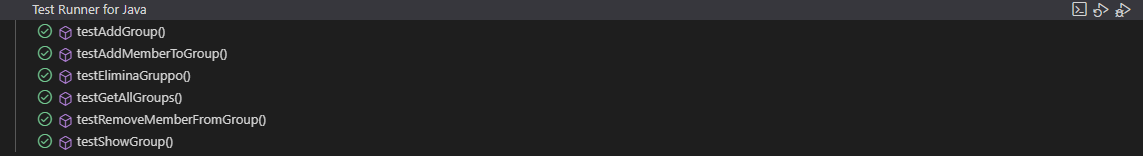
\includegraphics[width=0.9\textwidth]{images/TestGroupController.png}
    \caption{Test per la classe GroupController}
    \label{fig:GroupController_test}
\end{figure}


\subsubsection{API Esposte}

Questa sezione documenta le API principali del sistema \textbf{Spendly}, includendo autenticazione, gestione dei gruppi e visualizzazione. Ogni test verrà mostrato con un' \texttt{immagine dei risultati}.

\paragraph{Registrazione Utente}
\begin{itemize}
    \item \textbf{Endpoint:} \texttt{POST /account/register}
    \item \textbf{Descrizione:} Consente a un nuovo utente di registrarsi al sistema.
    \item \textbf{Parametri:}
    \begin{itemize}
        \item \texttt{nome} (string) - Nome utente.
        \item \texttt{cognome} (string) - Nome utente.
        \item \texttt{username} (string) - Username utente(non accetta duplicati).
        \item \texttt{email} (string) - Email dell'utente(non accetta duplicati).
        \item \texttt{telefono} (string) - Telefono utente.
        \item \texttt{indirizzo} (string) - Indirizzo utente.
        \item \texttt{password} (string) - Password scelta dall'utente.
    \end{itemize}
    \item \textbf{Risultato:}
\end{itemize}
\begin{figure}[H]
    \centering
    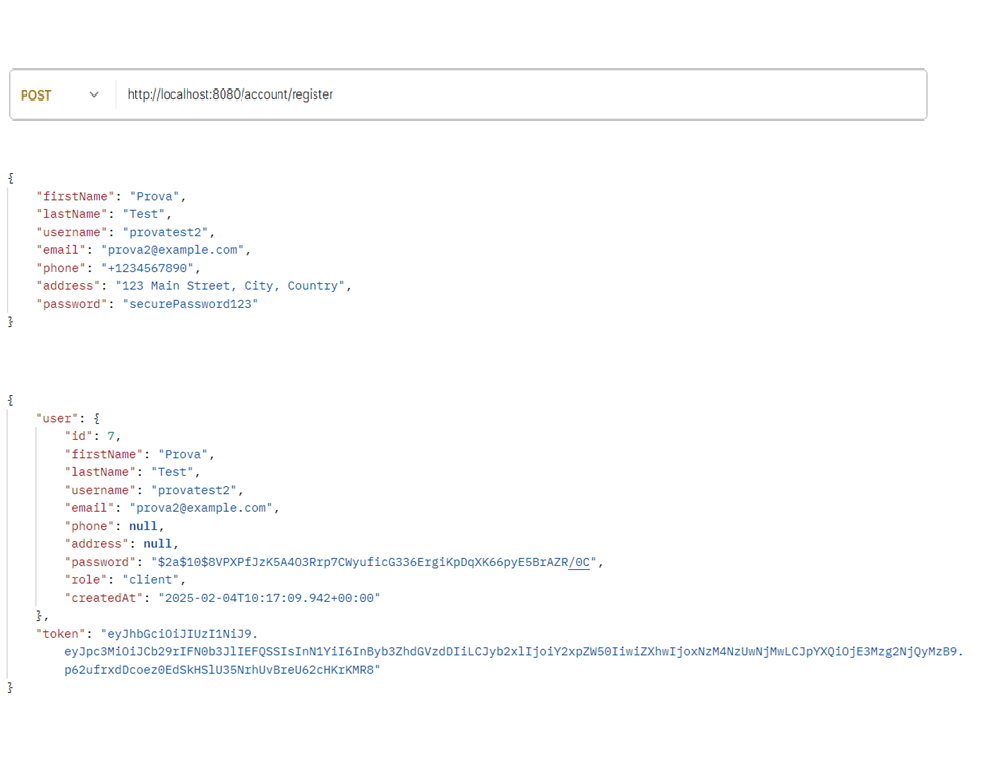
\includegraphics[width=0.9\textwidth]{images/registerapi.png}
    \caption{Risultato API Registrazione}
    \label{fig:api_register}
\end{figure}

\paragraph{Login Utente}
\begin{itemize}
    \item \textbf{Endpoint:} \texttt{POST /account/login}
    \item \textbf{Descrizione:} Permette a un utente registrato di accedere al sistema.
    \item \textbf{Parametri:}
    \begin{itemize}
        \item \texttt{username} (string) - Username dell'utente.
        \item \texttt{password} (string) - Password dell'utente.
    \end{itemize}
    \item \textbf{Risultato:}  
\end{itemize}
\begin{figure}[H]
    \centering
    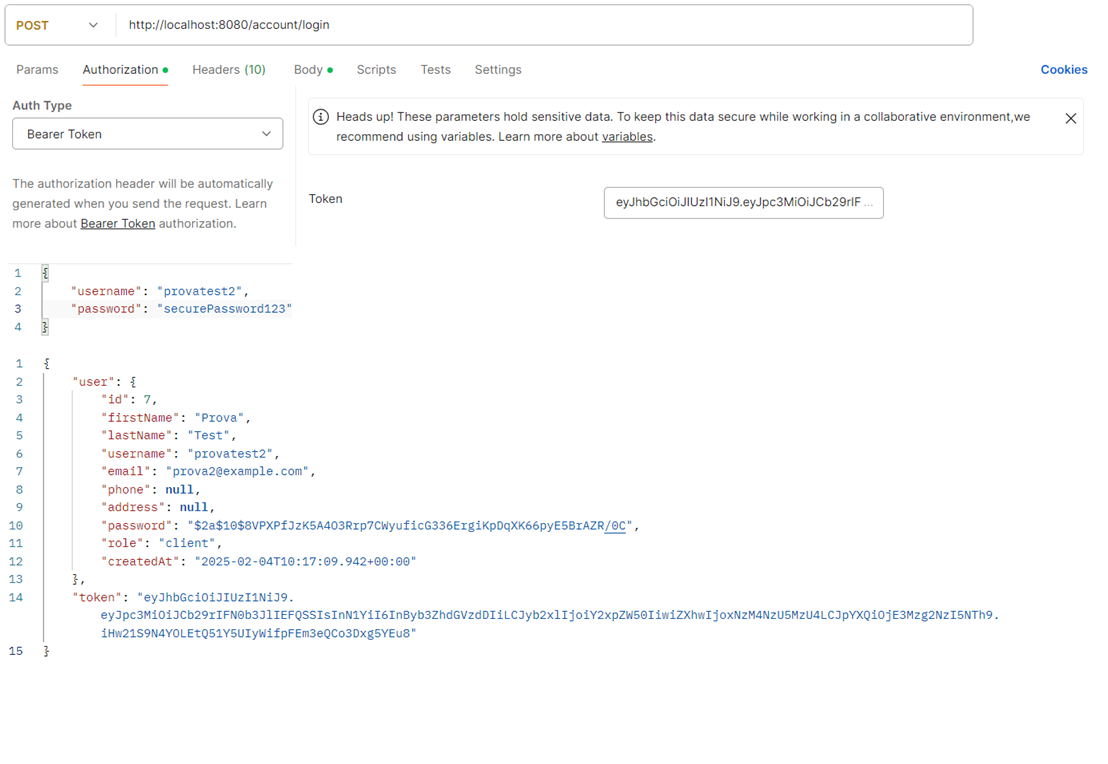
\includegraphics[width=0.9\textwidth]{images/loginapi.png}
    \caption{Risultato API Login}
    \label{fig:api_login}
\end{figure}

\paragraph{Creazione di un Gruppo}
\begin{itemize}
    \item \textbf{Endpoint:} \texttt{POST /api/groups}
    \item \textbf{Descrizione:} Permette la creazione di un nuovo gruppo da parte dell'utente.
    \item \textbf{Parametri:}
    \begin{itemize}
        \item \texttt{name} (string) - Nome del gruppo.
        \item \texttt{username} (string) - Username dell'utente che crea il gruppo.
    \end{itemize}
    \item \textbf{Risultato:}
\end{itemize}
\begin{figure}[H]
    \centering
    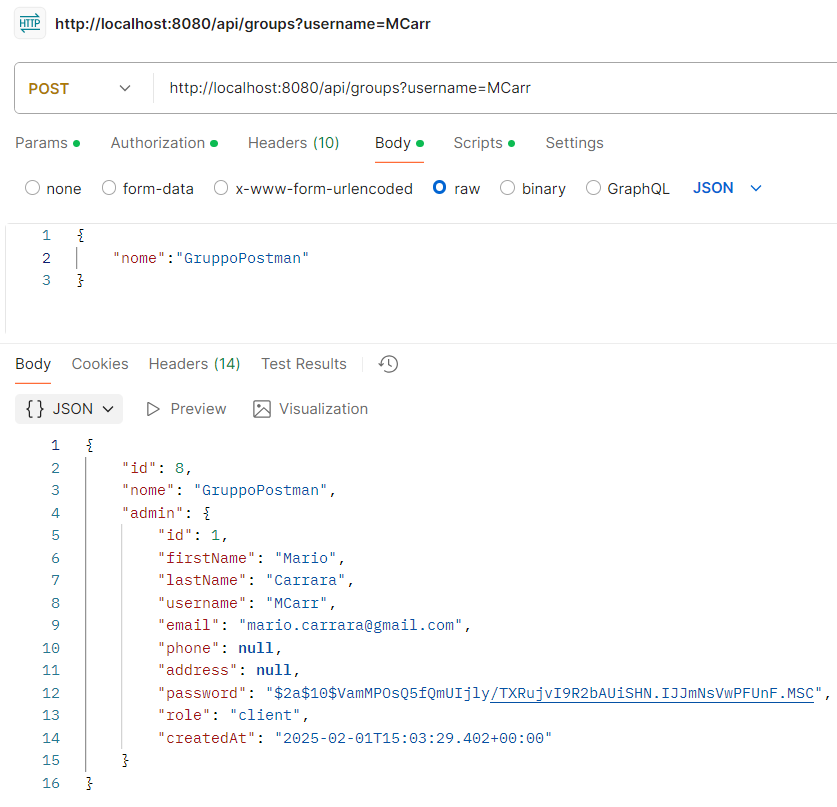
\includegraphics[width=0.8\textwidth]{images/CreateGroupAPI.png}
    \caption{Risultato API Creazione Gruppo}
    \label{fig:api_create_group}
\end{figure}

\paragraph{Inserimento di un utente in un gruppo}
\begin{itemize}
    \item \textbf{Endpoint:} \texttt{POST /api/groups/{group\_id}/members}
    \item \textbf{Descrizione:} Permette all'amministratore di inserire un utente in un gruppo.
    \item \textbf{Parametri:}
    \begin{itemize}
        \item \texttt{adminUsername} (string) - Username dell'admin del gruppo.
        \item \texttt{memberUsername} (string) - Username dell'utente da inserire.
    \end{itemize}
    \item \textbf{Risultato:}
\end{itemize}
\begin{figure}[H]
    \centering
    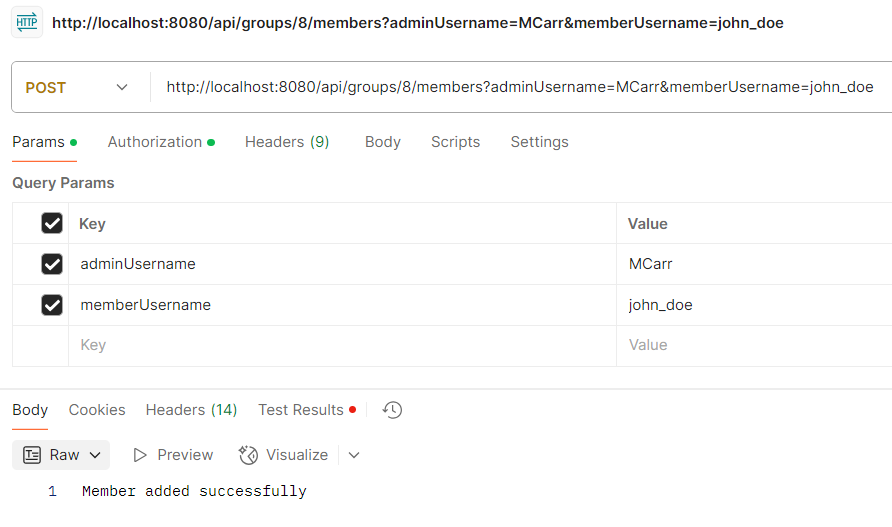
\includegraphics[width=0.8\textwidth]{images/AddMemberAPI.png}
    \caption{Risultato API Inserimento utente}
    \label{fig:api_add_member}
\end{figure}

\paragraph{Visualizzazione dei Gruppi}
\begin{itemize}
    \item \textbf{Endpoint:} \texttt{GET /api/groups}
    \item \textbf{Descrizione:} Restituisce la lista di tutti i gruppi a cui l'utente appartiene.
    \item \textbf{Parametri:}
    \begin{itemize}
        \item \texttt{username} (string) - Username dell'utente.
    \end{itemize}
    \item \textbf{Risultato:}
\end{itemize}
\begin{figure}[H]
    \centering
    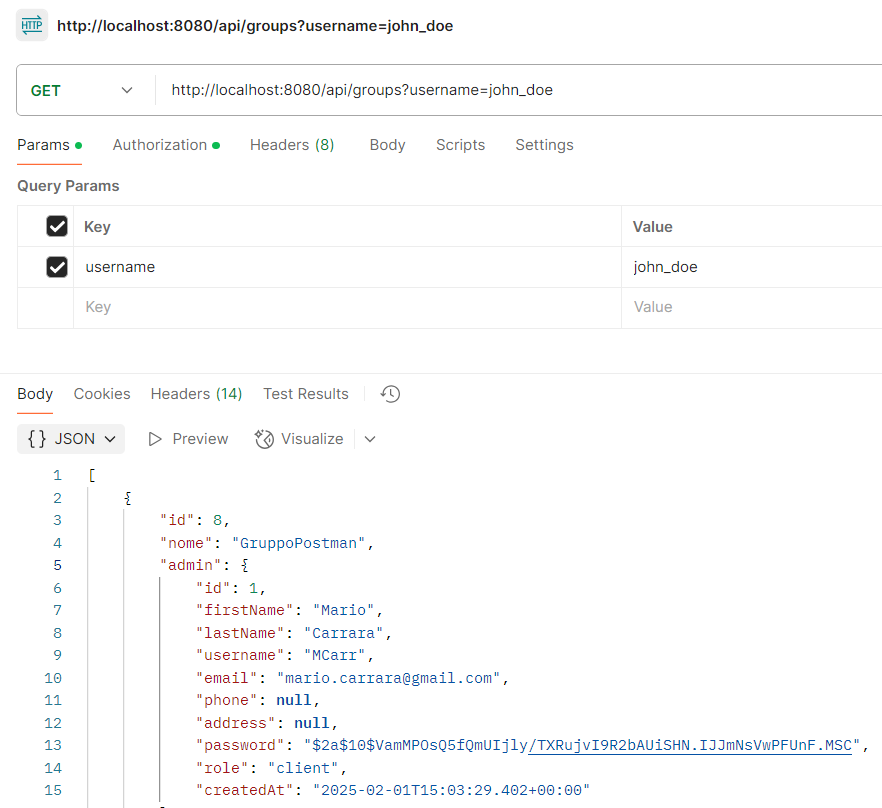
\includegraphics[width=0.8\textwidth]{images/GetAPI.png}
    \caption{Risultato API Visualizzazione Gruppi}
    \label{fig:api_view_groups}
\end{figure}



% =======================================================
% ITERAZIONE 2
% =======================================================
\newpage
\section{Iterazione 2}
\subsection{Casi d'Uso Implementati }

In questa iterazione sono stati sviluppati i seguenti casi d’uso ritenuti prioritari per lo sviluppo di \textbf{Spendly}.

\begin{table}[h]
    \centering
    \begin{tabular}{|c|l|}
    \hline
    \textbf{ID} & \textbf{Titolo} \\ \hline
    UC4 & Crea alert di gruppo\\ \hline
    UC5 & Modifica alert \\ \hline
    UC6 & Elimina alert \\ \hline
    UC12 & Accedi gruppo \\ \hline
    UC13 & Inserisci spesa \\ \hline
    UC14 & Elimina spesa \\ \hline
    UC15 & Modifica spesa \\ \hline
    UC16 & Visualizza spese \\ \hline
    UC17 & Ricalcolo debiti \\ \hline
    \end{tabular}
    \caption{Iterazione2}
\end{table}

\subsubsection{UC4: Creazione Alert di Gruppo}
\textbf{Attori}: Utente amministratore, Sistema.
\newline
\newline
\textbf{Descrizione}: L’amministratore di un gruppo può creare un alert per segnalare il raggiungimento di una soglia limite di spesa.
\newline
\newline
\textbf{Flusso degli eventi}:
\begin{enumerate}
    \item L’amministratore accede alla pagina del gruppo.
    \item Clicca su "Crea Alert".
    \item Inserisce il limite di spesa e una descrizione opzionale.
    \item Il sistema salva l’alert e lo associa al gruppo.
\end{enumerate}

\subsubsection{UC5: Modifica Alert}
\textbf{Attori}: Utente amministratore, Sistema.
\newline
\newline
\textbf{Descrizione}: L’amministratore di un gruppo può modificare i valori di un alert già impostato.
\newline
\newline
\textbf{Flusso degli eventi}:
\begin{enumerate}
    \item L’amministratore accede alla lista degli alert.
    \item Seleziona un alert e modifica i parametri (soglia limite, descrizione).
    \item Il sistema aggiorna le informazioni dell’alert.
\end{enumerate}

\subsubsection{UC6: Eliminazione Alert}
\textbf{Attori}: Utente amministratore, Sistema.
\newline
\newline
\textbf{Descrizione}: L’amministratore di un gruppo può eliminare un alert impostato in precedenza.
\newline
\newline
\textbf{Flusso degli eventi}:
\begin{enumerate}
    \item L’amministratore accede alla lista degli alert del gruppo.
    \item Seleziona un alert e clicca su "Elimina".
    \item Il sistema chiede conferma e poi rimuove l’alert.
\end{enumerate}

\subsubsection{UC13: Inserimento Spesa}
\textbf{Attori}: Utente, Sistema.
\newline
\newline
\textbf{Descrizione}: Un utente appartenente a un gruppo può aggiungere una spesa condivisa.
\newline
\newline
\textbf{Flusso degli eventi}:
\begin{enumerate}
    \item L’utente accede alla pagina del gruppo.
    \item Clicca su "Aggiungi Spesa".
    \item Inserisce l’importo, la descrizione e seleziona i partecipanti.
    \item Il sistema registra la spesa e aggiorna il bilancio del gruppo.
\end{enumerate}

\subsubsection{UC14: Eliminazione Spesa}
\textbf{Attori}: Utente, Sistema.
\newline
\newline
\textbf{Descrizione}: Un utente può eliminare una spesa precedentemente inserita.
\newline
\newline
\textbf{Flusso degli eventi}:
\begin{enumerate}
    \item L’utente accede alla lista delle spese del gruppo.
    \item Seleziona una spesa e clicca su "Elimina".
    \item Il sistema chiede conferma e poi rimuove la spesa dal gruppo.
\end{enumerate}

\subsubsection{UC15: Modifica Spesa}
\textbf{Attori}: Utente, Sistema.
\newline
\newline
\textbf{Descrizione}: Un utente può modificare i dettagli di una spesa condivisa nel gruppo.
\newline
\newline
\textbf{Flusso degli eventi}:
\begin{enumerate}
    \item L’utente accede alla lista delle spese.
    \item Seleziona una spesa e clicca su "Modifica".
    \item Modifica i dati della spesa (importo, descrizione, partecipanti).
    \item Il sistema aggiorna la spesa e ricalcola i bilanci.
\end{enumerate}

\subsubsection{UC16: Visualizzazione Spese}
\textbf{Attori}: Utente, Sistema.
\newline
\newline
\textbf{Descrizione}: Un utente può visualizzare tutte le spese del gruppo di cui fa parte.
\newline
\newline
\textbf{Flusso degli eventi}:
\begin{enumerate}
    \item L’utente accede alla pagina del gruppo.
    \item Clicca su "Visualizza Spese".
    \item Il sistema mostra l’elenco delle spese con dettagli su importo, data e partecipanti.
\end{enumerate}

\subsubsection{UC17: Ricalcolo Debiti}
\textbf{Attori}: Utente, Sistema.
\newline
\newline
\textbf{Descrizione}: Un utente può calcolare il riepilogo dei debiti tra i membri del gruppo.
\newline
\newline
\textbf{Flusso degli eventi}:
\begin{enumerate}
    \item L’utente accede alla pagina del gruppo.
    \item Clicca su "Calcola Debiti".
    \item Il sistema analizza le spese e genera un riepilogo dei debiti tra i membri.
    \item L’utente visualizza il riepilogo e le modalità di saldo consigliate.
\end{enumerate}



\newpage
\subsection{UML Component Diagram}


\begin{center}
    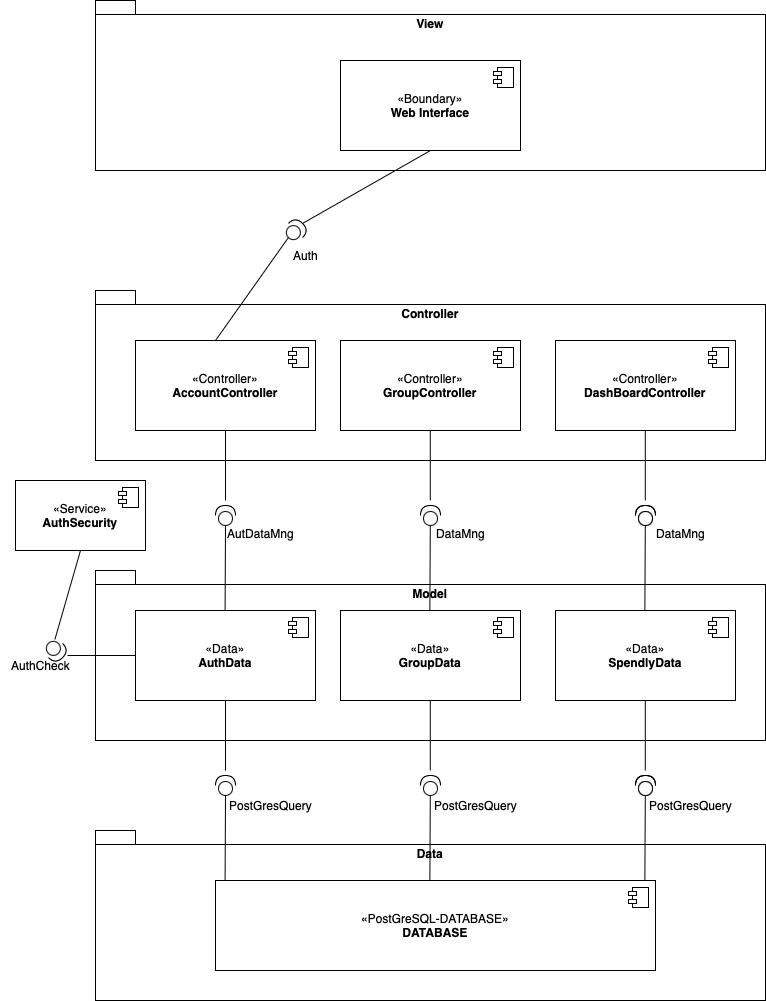
\includegraphics[scale=0.45]{images/ComponentDiagramV1.1.png}

\end{center}

Partendo dai casi d’uso selezionati per questa iterazione e procedendo con l’utilizzo delle euristiche di design, è stato possibile progettare l’architettura software del sistema \textbf{Spendly}.  
I componenti sono organizzati secondo il pattern \textbf{MVC (Model-View-Controller)}, con la suddivisione in:
\begin{itemize}
    \item \textbf{Boundary} - Interfaccia utente, responsabile dell'interazione con l'utente finale.
    \item \textbf{Controller} - Gestione logica di business.
    \item \textbf{Model} - Gestione dei dati e accesso al database.
    \item \textbf{Service} - Servizi di sicurezza e autenticazione.
    \item \textbf{Database} - PostgreSQL.
\end{itemize}

\newpage
\subsection{UML Class Diagram per tipi di dato}
%spazio
\hspace{35pt}
\begin{center}
    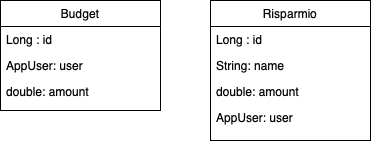
\includegraphics[scale=0.85]{images/DiagrammaClassiTipoDatoBudgetRisparmio.png}
\end{center}




\newpage
\subsection{Testing}
\subsubsection{Analisi Statica - CodeMR}

\begin{figure}[H]
    \centering
    \begin{minipage}{0.45\textwidth}
        \centering
        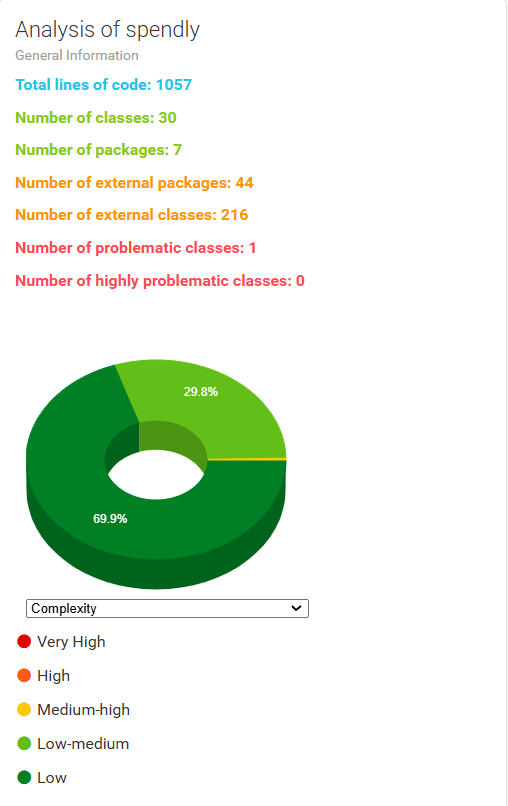
\includegraphics[width=\textwidth]{images/Complexity_iter2.png}
        \caption{Complexity}
        \label{fig:Complexity_iterazione2}
    \end{minipage}
    \hfill
    \begin{minipage}{0.45\textwidth}
        \centering
        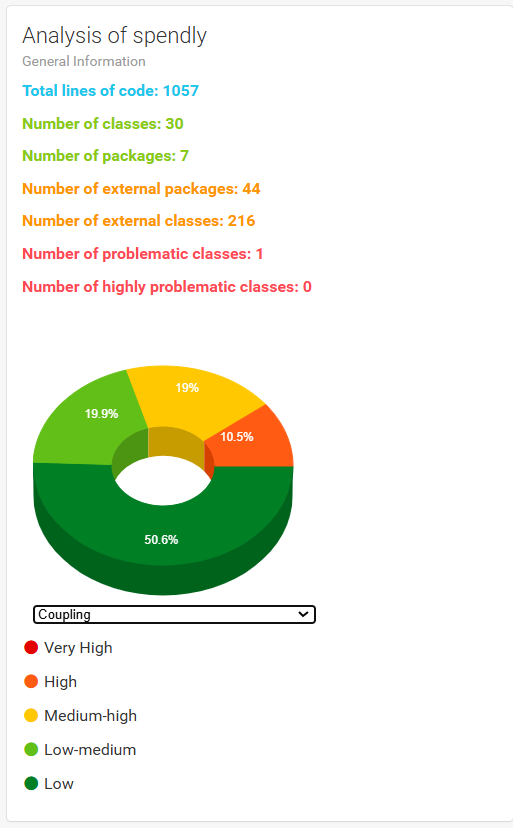
\includegraphics[width=\textwidth]{images/Coupling_iter2.png}
        \caption{Coupling}
        \label{fig:Coupling_iterazione2}
    \end{minipage}
\end{figure}

\begin{figure}[H]
    \centering
    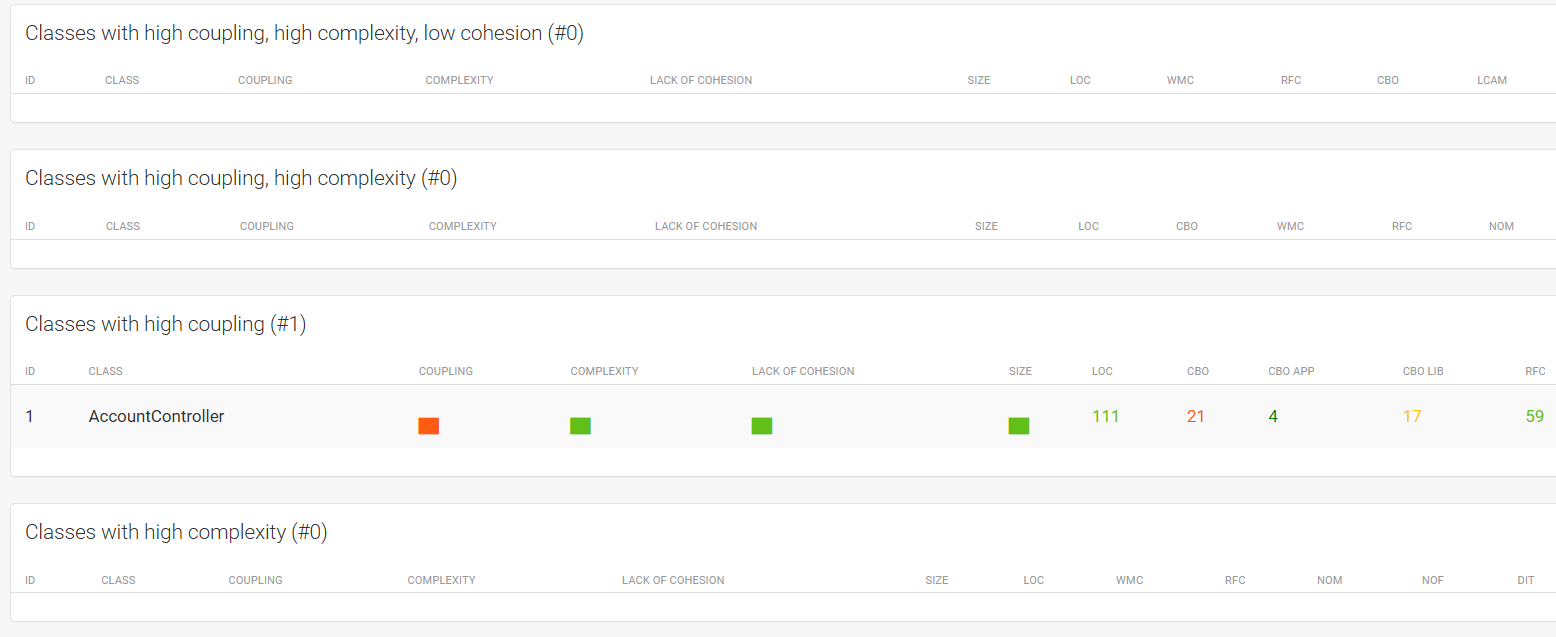
\includegraphics[width=0.9\textwidth]{images/Problem_iter2.png}
    \caption{Problemi classi}
    \label{fig:Problemi_iterazione2}
\end{figure}


\begin{figure}[H]
    \centering
    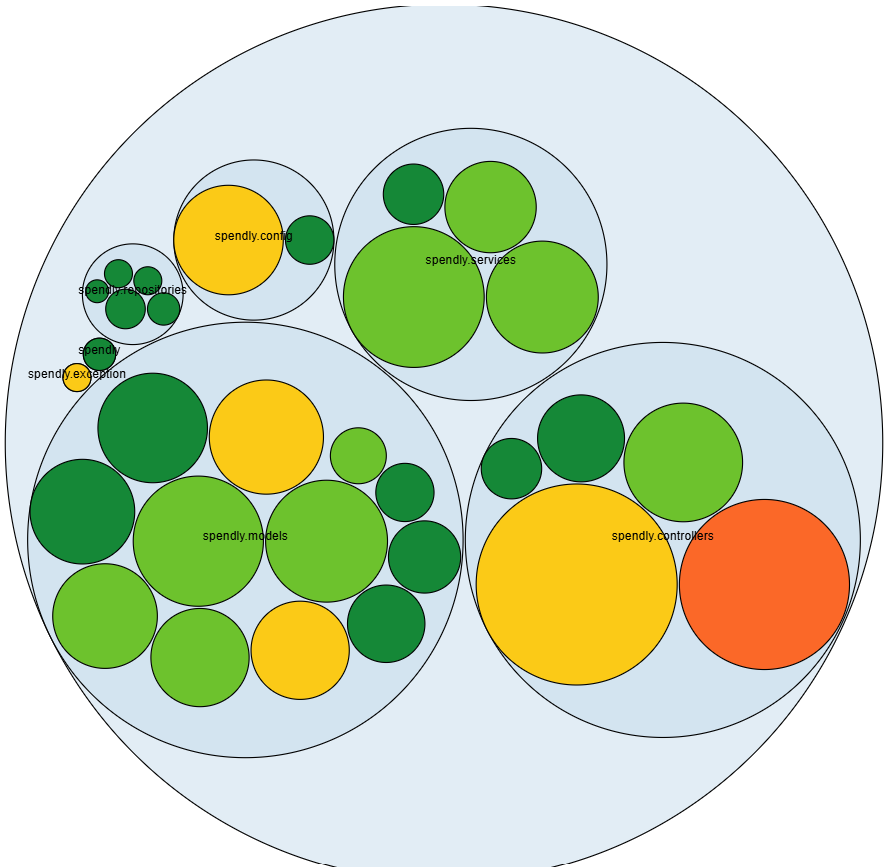
\includegraphics[width=0.8\textwidth]{images/Package_iter2.png}
    \caption{Struttura dei package}
    \label{fig:Package_iterazione2}
\end{figure}

\subsubsection{Analisi Dinamica - JUnit}

\begin{figure}[H]
    \centering
    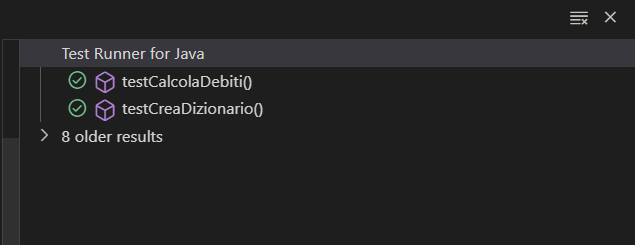
\includegraphics[width=0.9\textwidth]{images/CalcolaDebitiTest.png}
    \caption{Test per ottimizzare Debiti}
    \label{fig:CalcolaDebitiTest}
\end{figure}

\begin{figure}[H]
    \centering
    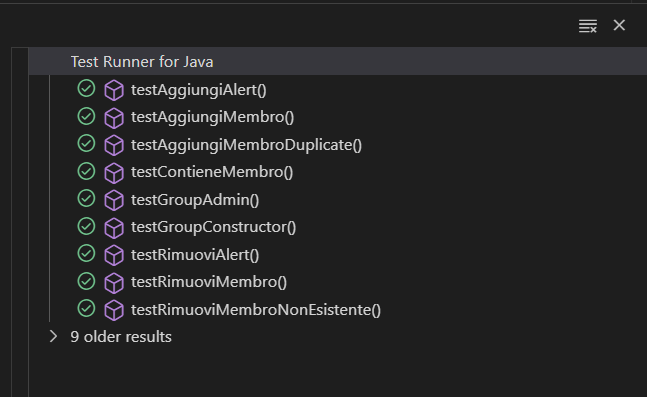
\includegraphics[width=0.9\textwidth]{images/GroupTest_iter2.png}
    \caption{Test aggiornati per la classe Group}
    \label{fig:GroupTest_iter2}
\end{figure}

\begin{figure}[H]
    \centering
    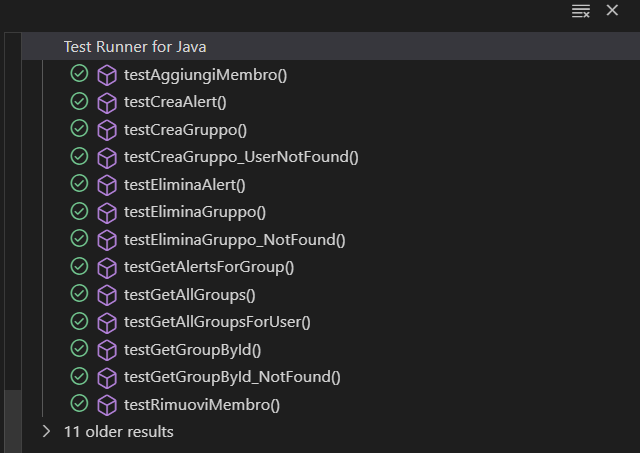
\includegraphics[width=0.9\textwidth]{images/GroupServiceTest_iter2.png}
    \caption{Test aggiornati per la classe GroupService}
    \label{fig:GroupServiceTest_iter2}
\end{figure}

\begin{figure}[H]
    \centering
    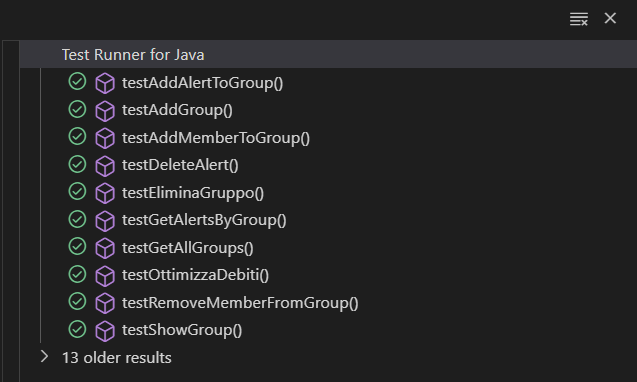
\includegraphics[width=0.9\textwidth]{images/GroupControllerTest_iter2.png}
    \caption{Test aggiornati per la classe GroupController}
    \label{fig:GroupControllerTest_iter2}
\end{figure}

\begin{figure}[H]
    \centering
    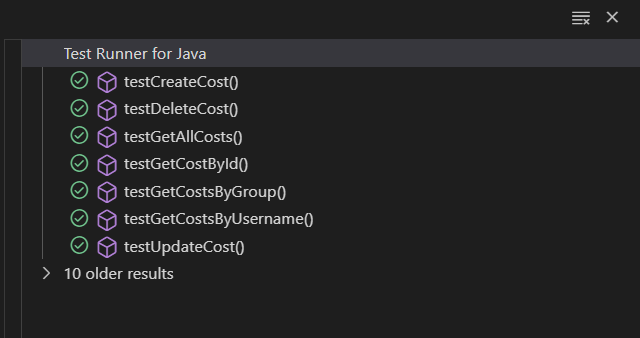
\includegraphics[width=0.9\textwidth]{images/CostServiceTest_iter2.png}
    \caption{Test per la classe CostService}
    \label{fig:GroupControllerTest_iter2}
\end{figure}

\begin{figure}[H]
    \centering
    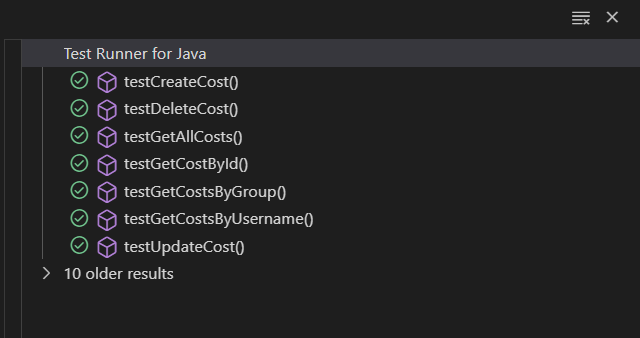
\includegraphics[width=0.9\textwidth]{images/CostServiceTest_iter2.png}
    \caption{Test per la classe CostService}
    \label{fig:CostServiceTest_iter2}
\end{figure}

\begin{figure}[H]
    \centering
    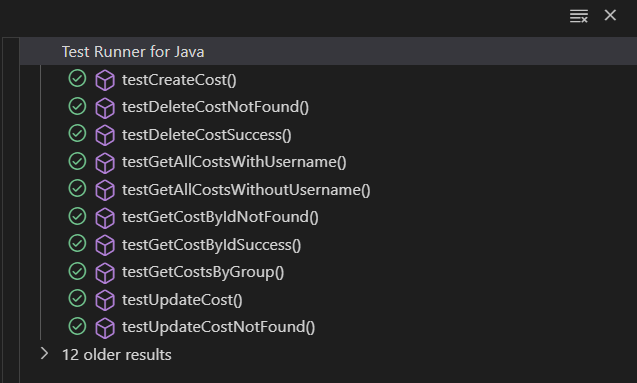
\includegraphics[width=0.9\textwidth]{images/CostControllerTest_iter2.png}
    \caption{Test per la classe CostController}
    \label{fig:CostControllerTest_iter2}
\end{figure}



\subsubsection{API Costi}

Questa sezione documenta le API relative alla gestione dei **costi** nel sistema **Spendly**, inclusi la creazione, l'eliminazione e la visualizzazione dei costi di utenti e gruppi. Ogni test verrà mostrato con un'**immagine dei risultati**.

\paragraph{Aggiunta di un Costo}  

\begin{itemize}
    \item \textbf{Endpoint:} \texttt{POST /api/costs?username=\{username\}}
    \item \textbf{Descrizione:} Permette all'utente autenticato di aggiungere un nuovo costo, eventualmente associandolo a un gruppo.
    \item \textbf{Parametri:}
    \begin{itemize}
        \item \texttt{importo} (double) - Importo della spesa.
        \item \texttt{tipologia} (string) - Tipo di spesa.
        \item \texttt{groupId} (integer, opzionale) - ID del gruppo a cui associare il costo.
    \end{itemize}
\end{itemize}
\newpage
\begin{figure}[h!]
    \centering
    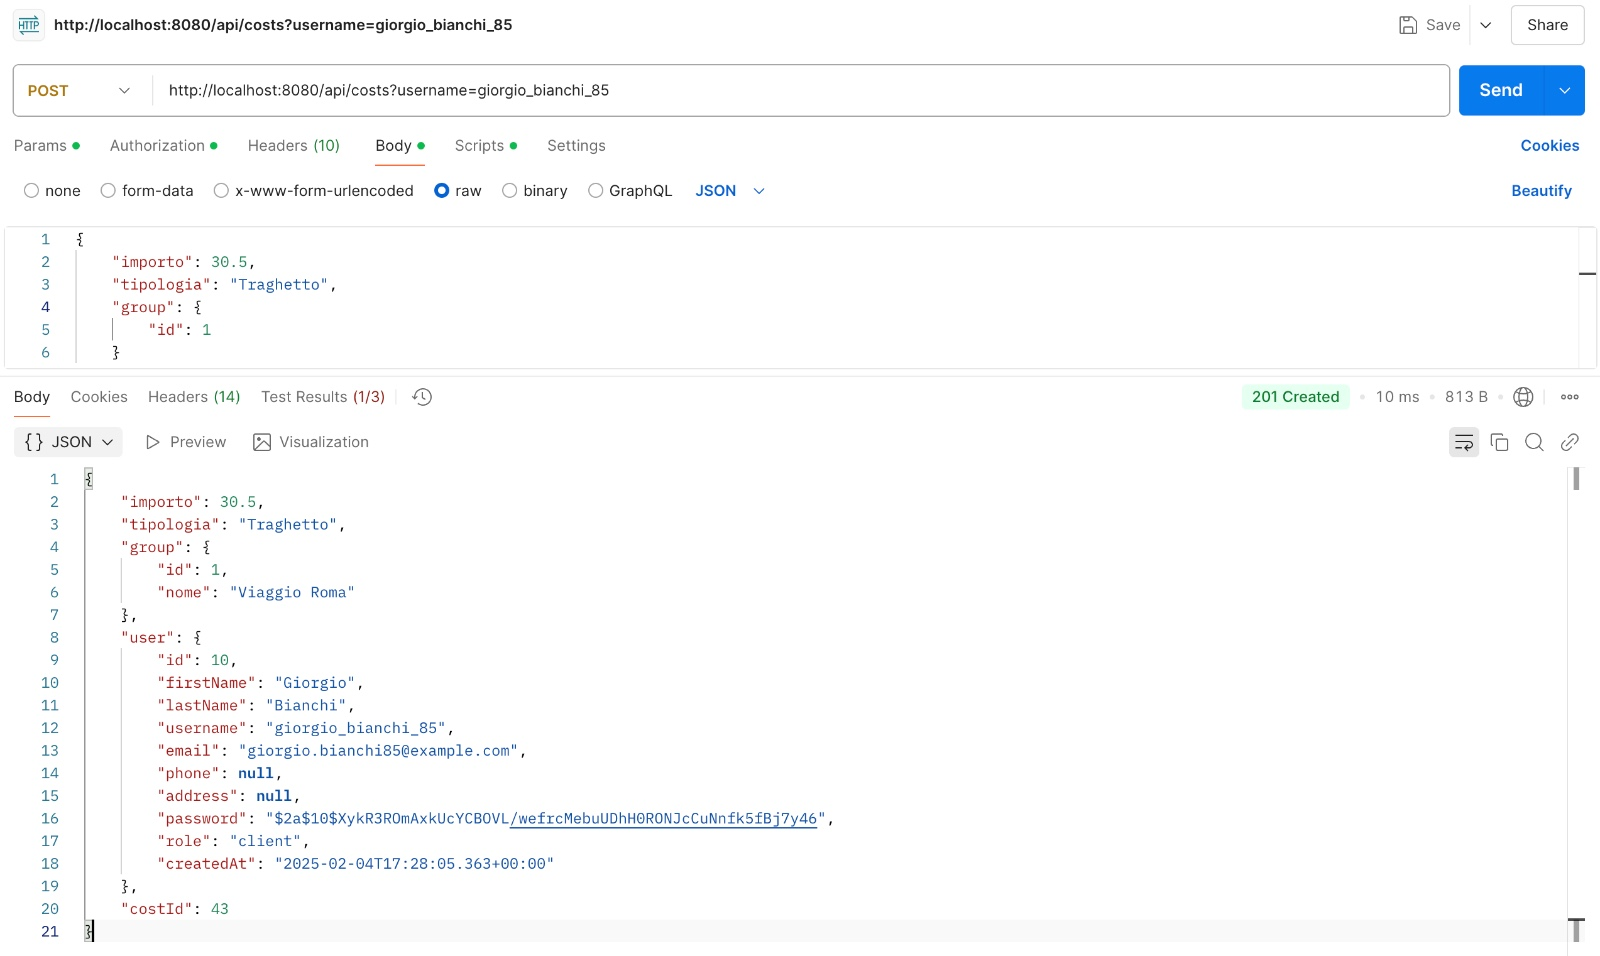
\includegraphics[width=0.9\textwidth]{images/createCost.jpeg}
    \caption{Risultato API Aggiunta Costo}
    \label{fig:api_add_cost}
\end{figure}

\paragraph{Eliminazione di un Costo}  

\begin{itemize}
    \item \textbf{Endpoint:} \texttt{DELETE /api/costs/\{costId\}}
    \item \textbf{Descrizione:} Permette all'utente autenticato di eliminare un costo precedentemente registrato.
    \item \textbf{Parametri:}
    \begin{itemize}
        \item \texttt{\{costId\}} (integer) - ID del costo da eliminare.
    \end{itemize}
\end{itemize}

\begin{figure}[h!]
    \centering
    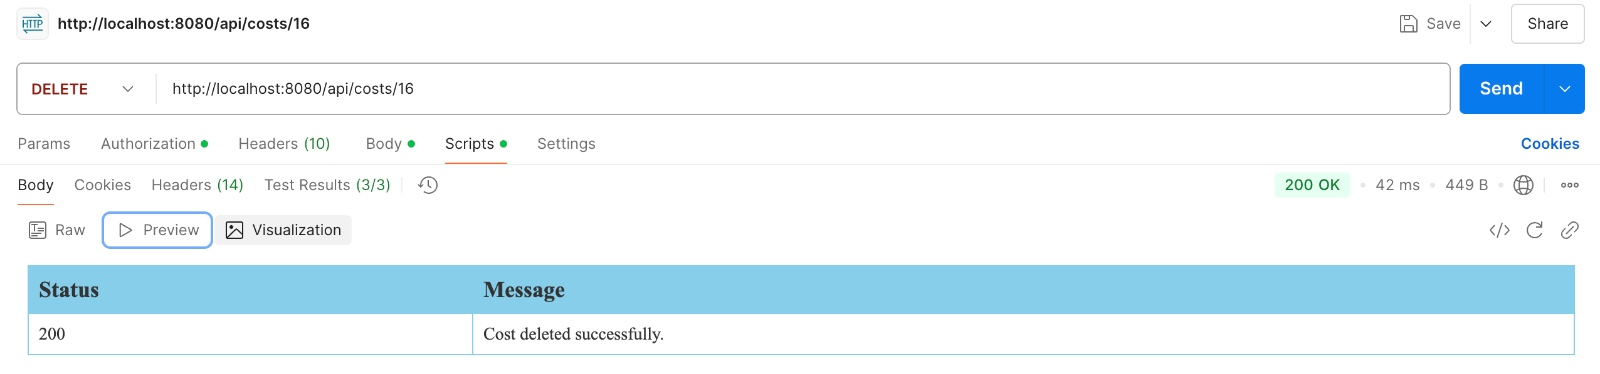
\includegraphics[width=0.9\textwidth]{images/deleteCost.jpeg}
    \caption{Risultato API Eliminazione Costo}
    \label{fig:api_delete_cost}
\end{figure}

\paragraph{Visualizzazione Costi Utente}  

\begin{itemize}
    \item \textbf{Endpoint:} \texttt{GET /api/costs?username=\{username\}}
    \item \textbf{Descrizione:} Restituisce la lista di tutti i costi registrati dall'utente autenticato.
\end{itemize}

\begin{figure}[h!]
    \centering
    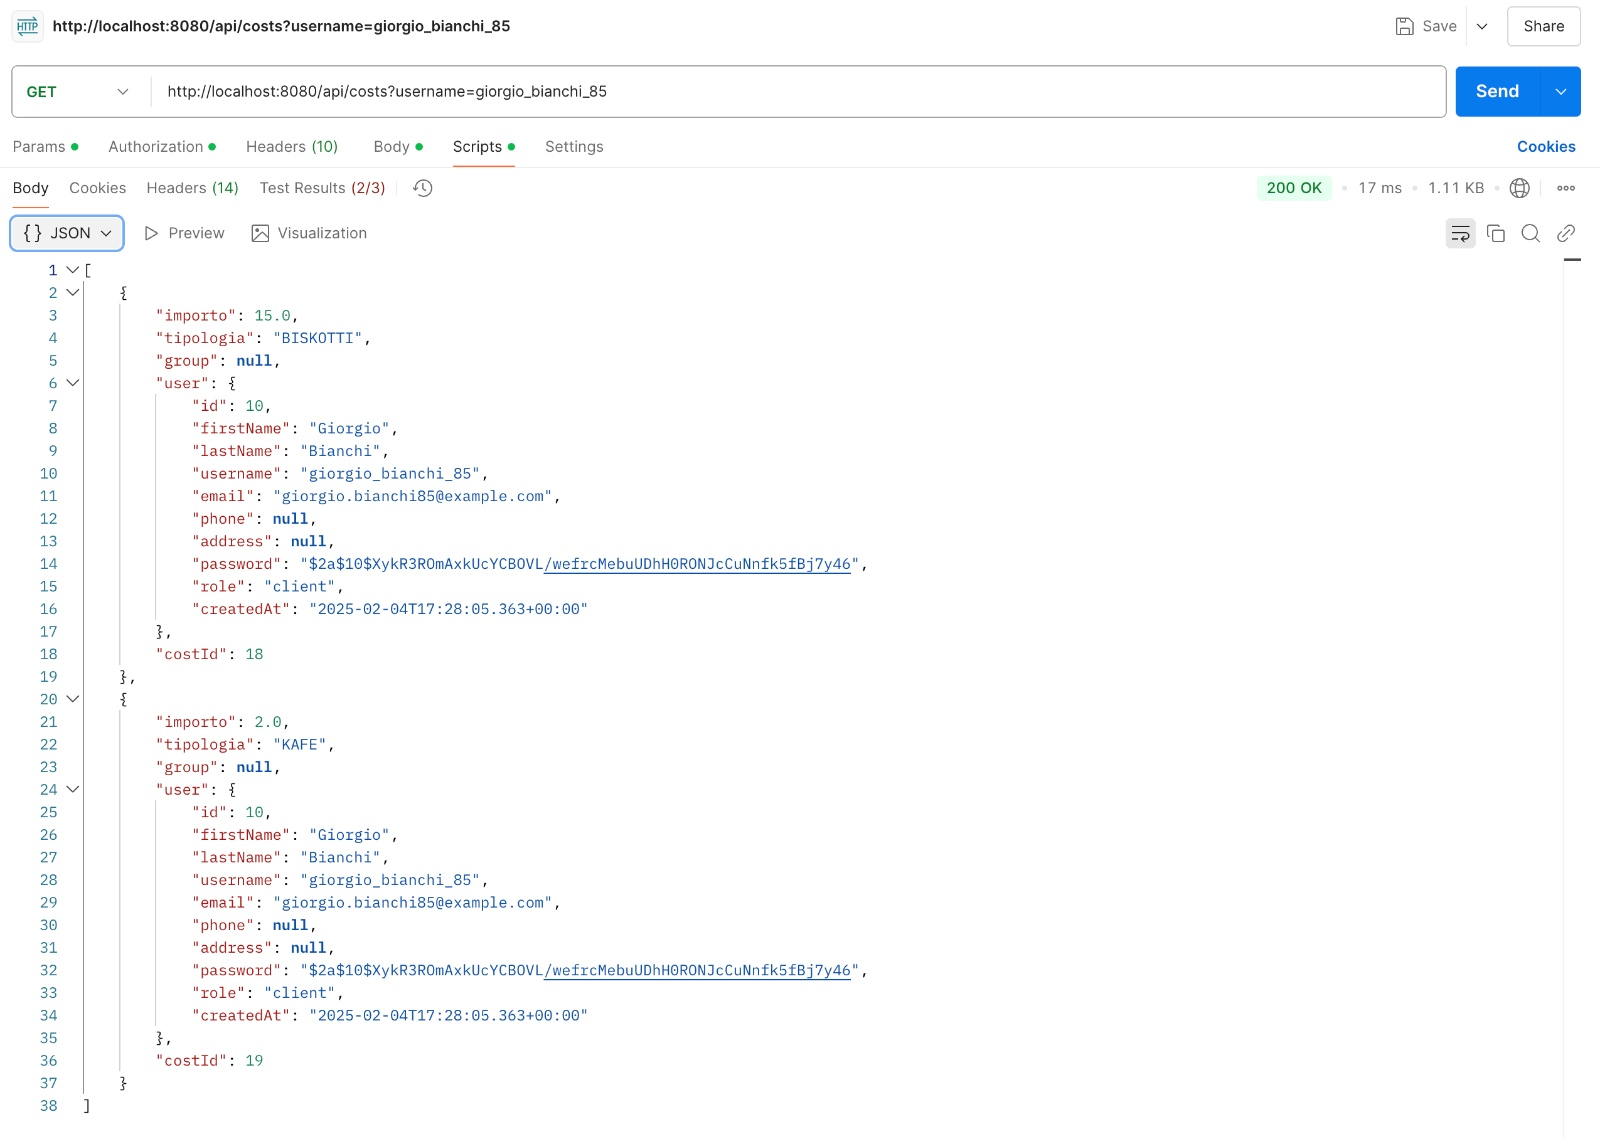
\includegraphics[width=0.9\textwidth]{images/getUserCosts.jpeg}
    \caption{Risultato API Visualizzazione Costi Utente}
    \label{fig:api_view_user_costs}
\end{figure}

\paragraph{Visualizzazione Costi di un Gruppo}  

\begin{itemize}
    \item \textbf{Endpoint:} \texttt{GET /api/costs/group/\{groupId\}}
    \item \textbf{Descrizione:} Restituisce la lista di tutti i costi registrati del gruppo.
\end{itemize}

\begin{figure}[H]
    \centering
    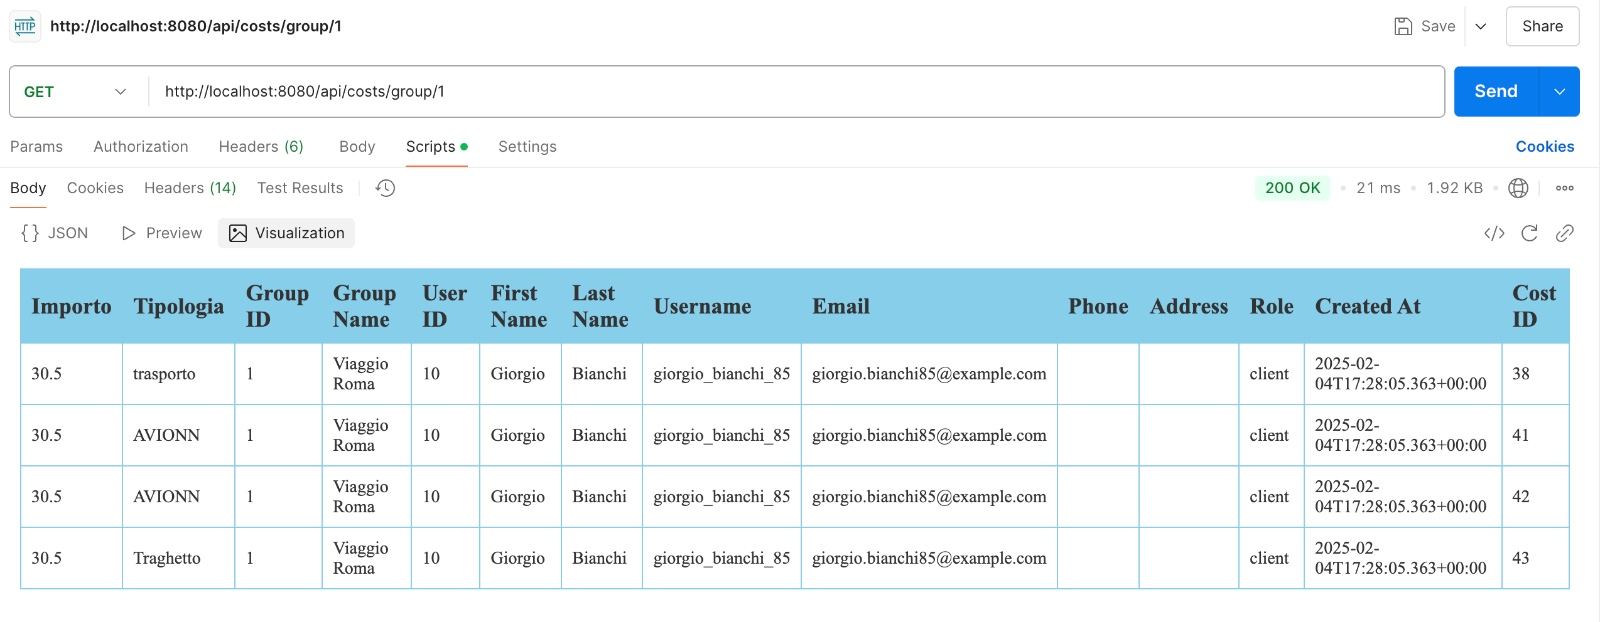
\includegraphics[width=0.9\textwidth]{images/getGroupCosts.jpeg}
    \caption{Risultato API Visualizzazione Costi Gruppo}
    \label{fig:api_view_group_costs}
\end{figure}


\paragraph{Creazione Alert} 

\begin{itemize}
    \item \textbf{Endpoint:} \texttt{POST /api/groups/\{groupId\}/alerts?username=\{username\}}
    \item \textbf{Descrizione:} Permette all'amministratore del gruppo di creare un Alert
\end{itemize}

\begin{figure}[H]
    \centering
    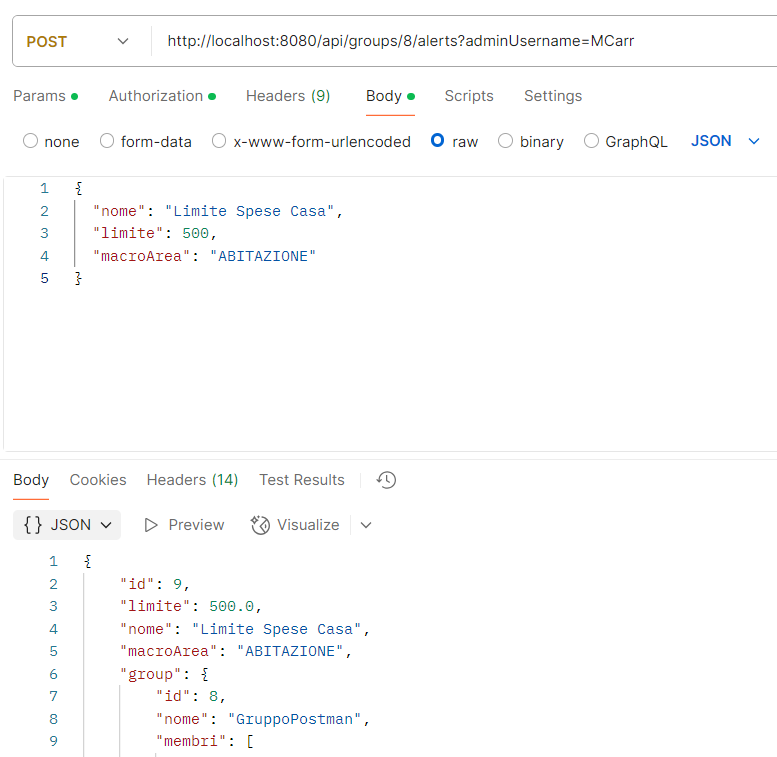
\includegraphics[width=0.9\textwidth]{images/createAlert.png}
    \caption{Risultato API Creazione Alert}
    \label{fig:api_createAlert}
\end{figure}

\paragraph{Eliminazione Alert}

\begin{itemize}
    \item \textbf{Endpoint:} \texttt{DELETE /api/groups/{groupId}/alerts/{alertId}?username={username}}
    \item \textbf{Descrizione:} Permette all'amministratore del gruppo di eliminare un Alert.
\end{itemize}

\begin{figure}[H]
    \centering
    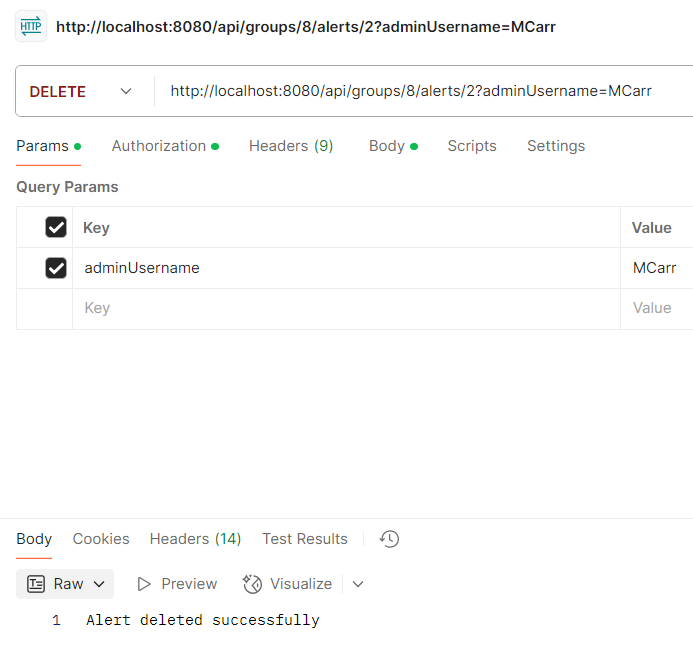
\includegraphics[width=0.9\textwidth]{images/DeleteAlert.png}
    \caption{Risultato API eliminazione Alert}
    \label{fig:api_deleteAlert}
\end{figure}

\paragraph{Visualizza Alert di Gruppo}

\begin{itemize}
    \item \textbf{Endpoint:} \texttt{GET /api/groups/{groupId}/alerts}
    \item \textbf{Descrizione:} Restituisce la lista di tutti gli alerts del gruppo.
\end{itemize}

\begin{figure}[H]
    \centering
    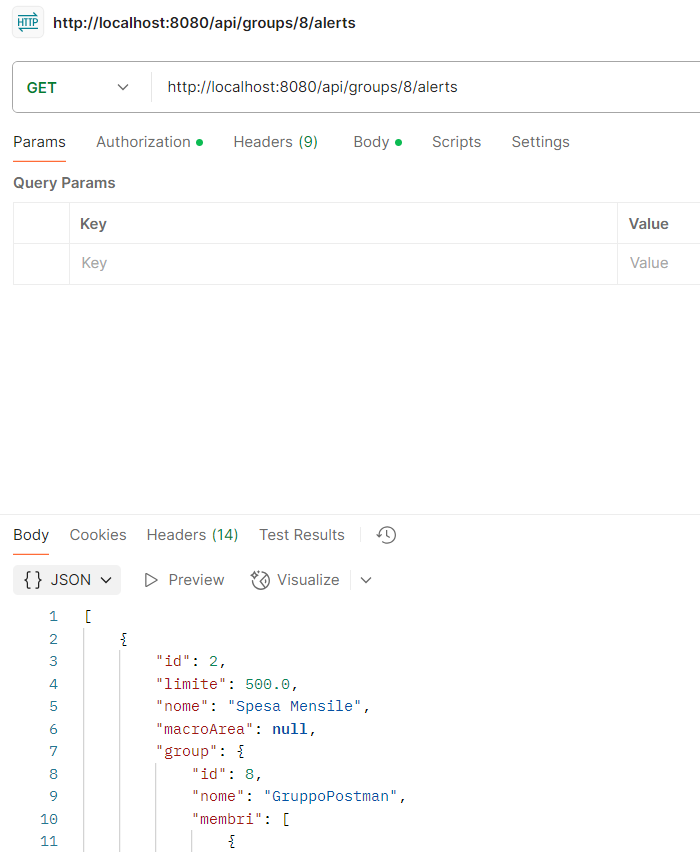
\includegraphics[width=0.9\textwidth]{images/GetAlertsForGroup.png}  
    \caption{Risultato API Visualizzazione Alert di Gruppo}
    \label{fig:api_view_group_alerts}  
\end{figure}


\end{document}